%instiki:category: FisicaSubatomica
\chapter{Modelo Est\'andar}
\label{cha:modelo-estandar} %noinstiki
%instiki:
%instiki:***
%instiki:
%instiki:[[NotasFS|Tabla de Contenidos]]
%instiki:
%instiki:***
%instiki:
%instiki:* [Interacci\'on Electrod\'ebil](#inter-electr)
%instiki:
%instiki:* [Modelo Est\'andar](#modelo-estandar)
%instiki:
%instiki:***
%instiki:

\section{Contenido de partículas}

\begin{frame}[fragile,allowframebreaks]
The known matter is build from the elementary set of particles defined in table
\begin{table}
  \centering
  \begin{tabular}{l|l|c|r}
    Type &Name & Symbol&Charge\\\hline{}
   leptons& electron & $e$& $-1$\\
          & neutrino & $\nu$ & $0$\\\hline{}
   quarks &up quark & $u_1,u_2,u_3$ & $2/3$\\
          &down quark & $d_1,d_2,d_3$& $-1/3$\\
  \end{tabular}
  \caption{Elementary fermions. The symbol represent both the particle, e.g $e^-$, as the antiparticle, e.g, $e^+$. The lectric chage is given in units of the electron chage $e$  }
  \label{tab:ef}
\end{table}

we further define the color triplets of quarks as
\begin{align}
  u=&
  \begin{pmatrix}
    u_1 \\ u_2\\ u_3\\
  \end{pmatrix}
  &d=&
  \begin{pmatrix}
    d_1 \\ d_2 \\ d_3\\
  \end{pmatrix}
\end{align}


The free Lagrangian containing this particles can be written as
\begin{align}
  \mathcal{L}_{\text{free}}=&i\overline{e}\gamma^\mu\partial_\mu e-m_e\overline{e}e+i\overline{\nu}\gamma^\mu\partial_\mu\nu
+i\overline{u}\gamma^\mu\partial_\mu u-m_u\overline{u}u+i\overline{d}\gamma^\mu\partial_\mu d-m_d\overline{d}d\nonumber\\
=&i\overline{e_L}\gamma^\mu\partial_\mu e_L+i\overline{e_R}\gamma^\mu\partial_\mu e_R-m_e(\overline{e_R}e_L+\overline{e_L}e_R)+i\overline{\nu_L}\gamma^\mu\partial_\mu\nu_L\nonumber\\
&+i\overline{\nu_R}\gamma^\mu\partial_\mu\nu_R+i\overline{u_L}\gamma^\mu\partial_\mu u_L+i\overline{u_R}\gamma^\mu\partial_\mu u_R\nonumber\\
&-m_e(\overline{u_R}u_L+\overline{u_L}u_R)
i\overline{d_L}\gamma^\mu\partial_\mu d_L+i\overline{d_R}\gamma^\mu\partial_\mu d_R-m_e(\overline{d_R}d_L+\overline{d_L}d_R)\,.
\end{align}
donde,
\begin{align}
  \nu_{L,R}=&P_{L,R}\nu,& e_{L,R}=&P_{L,R}\,e\nonumber\\
  u_{L,R}=&P_{L,R}\,u,& d_{L,R}=&P_{L,R}\,d\,.
\end{align}

\subsection*{Corrientes V--A}
\label{sec:corrientes-v}
En las interacciones débiles sólo participan las partes izquierdas de los campos. Esto nos permite prescindir del $\nu_R$, pues no tiene carga eléctrica, fuerte, o débil
\begin{align}
  \mathcal{L}_{\text{free}}
=&i\overline{e_L}\gamma^\mu\partial_\mu e_L+i\overline{e_R}\gamma^\mu\partial_\mu e_R-m_e(\overline{e_R}e_L+\overline{e_L}e_R)+
i\overline{\nu_L}\gamma^\mu\partial_\mu\nu_L\nonumber\\
&+i\overline{u_L}\gamma^\mu\partial_\mu u_L+i\overline{u_R}\gamma^\mu\partial_\mu u_R\nonumber\\
&-mue(\overline{u_R}u_L+\overline{u_L}u_R)+
i\overline{d_L}\gamma^\mu\partial_\mu d_L+i\overline{d_R}\gamma^\mu\partial_\mu d_R-m_d(\overline{d_R}d_L+\overline{d_L}d_R)\,.
\end{align}


\subsection*{Simetría global $SU(3)_c\times  SU(2)_L\times  U(1)_Y$}
\label{sec:simetr-glob-su2_l}

En el contexto de las interacciones débiles un $e_L$ es completamente equivalente a un campo $\nu_L$. Es decir, el Lagrangiano debe ser invariante bajo una transformación $SU(2)_L$ de esos campos. La diferencia entre ellos son sus respectivas cargas electricas y sus masas. Asumiendo que ambos campos tienen una misma hipercarga, asociada a una nueva simetría Abeliana $U(1)_Y$, podríamos esperar que la corriente electromagnética apropiada pueda obtenerse a partir del Grupo semisimple $SU(2)_L\times  U(1)_Y$. Además las respectivas masas se podrían obtener a partir del mecanismo de Higgs. 

La simetría $SU(2)_L$ entre las partes izquierdas del neutrino y el electrón, y entre las partes izquierdas de los quarks up y down, se establece  definiendo los dobletes:
  \begin{align}
    L\equiv\begin{pmatrix}
      \nu_L\\
      e_L      
    \end{pmatrix}\qquad   Q=&\begin{pmatrix}
    u_L\\
    d_L
  \end{pmatrix}\,,
  \end{align}
De otro lado, La invarianza bajo $U(1)_Y$ requiere que
\begin{align}
  Y_L=&Y_{\nu_L}=Y_{e_L}\nonumber\\
  Y_Q=&Y_{u_L}=Y_{d_L}\,.
\end{align}
El generador de carga eléctrica $\widehat{Q}$, se va obtener a partir de una combinación lineal del generador diagonal de $SU(2)_L$, $T_3$, y del generador de hipercarga, $Y$.

Bajo la simetría $SU(2)_L$, los campos transforman como:
 \begin{align}
  L\to L'=&\exp(i T^i \theta_i)L\approx(1+i T^i\theta_i)L\nonumber\\
  Q\to Q'=&\exp(i T^i \theta_i)Q\approx(1+i T^i\theta_i)Q\nonumber\\
  e_R\to& e'_R=e_R\nonumber\\
  u_R\to& u'_R=u_R\nonumber\\
  d_R\to& d'_R=d_R\,.
\end{align}
donde
\begin{align}
  T^i=\frac{\tau^i}{2}\,,
\end{align}
y $\tau^i$ son las matrices de Pauli dadas en la ec.~\eqref{eq:paulimatr}.

Claramente el término de masa $m_e$ en la ec.~(\ref{eq:261qft}) no es invariante bajo la simetría $SU(2)_L$. El Lagrangiano en la ec.~(\ref{eq:261qft}), sin término de masa, puede reescribirse de manera que exhíba de forma más explicita la invarianza bajo $SU(2)_L$ como
\begin{align}
  \mathcal{L}_{\text{free}}
=&i\overline{e_L}\gamma^\mu\partial_\mu e_L+i\overline{e_R}\gamma^\mu\partial_\mu e_R+i\overline{\nu_L}\gamma^\mu\partial_\mu\nu_L\nonumber\\
&+i\overline{u_L}\gamma^\mu\partial_\mu u_L+i\overline{u_R}\gamma^\mu\partial_\mu u_R
+i\overline{d_L}\gamma^\mu\partial_\mu d_L+i\overline{d_R}\gamma^\mu\partial_\mu d_R\nonumber\\
=&i\overline{L}\gamma^\mu\partial_\mu L+i\overline{Q}\gamma^\mu\partial_\mu Q+i\overline{e_R}\gamma^\mu\partial_\mu e_R
+i\overline{u_R}\gamma^\mu\partial_\mu u_R
+i\overline{d_R}\gamma^\mu\partial_\mu d_R\,.
\end{align}


\subsection*{Simetría gauge local $SU(3)_c\times  SU(2)_L\times  U(1)_Y$}

Para obtener la interacciones del modelo estándar, reemplazamos las derivadas normales por derivadas covariantes.

Proponemos entonces el Lagrangiano
\begin{align}
     \mathcal{L}=&i\overline{Q}\gamma^\mu\mathcal{D}_\mu Q+i\overline{L}\gamma^\mu\mathcal{D}_\mu L+
i\overline{e_R}\gamma^\mu\mathcal{D}_\mu {e_R}+i\overline{d_R}\gamma^\mu\mathcal{D}_\mu {d_R}+i\overline{u_R}\gamma^\mu\mathcal{D}_\mu {u_R}
\nonumber\\
     &-\tfrac{1}{4}G^{\mu\nu}_a G_{\mu\nu}^a-\tfrac{1}{4}W^{\mu\nu}_i W_{\mu\nu}^i-\tfrac{1}{4}B^{\mu\nu} B_{\mu\nu}\,,
\end{align}
Donde
\begin{align}
  \mathcal{D}^\mu&\equiv\partial^\mu-i g_s\frac{\lambda^a}{2}G^\mu_a-i g \frac{\tau^i}{2}W^\mu_i-i g'YB^\mu\,.
\end{align}
donde
\begin{align*}
  \Lambda^a\equiv\frac{\lambda^a}{2},\ a=1,2,\ldots,8 &\qquad\text{8 generadores de $SU(3)_c$}\\
  T^i\equiv\frac{\tau^i}{2},\ i=1,2,3 &\qquad\text{3 generadores de $SU(2)_L$}\\
  Y &\qquad\text{generador de $U(1)_Y$}
\end{align*}

All the particles in this Lagrangian are massless. It is only good for the gluons and the Abelian gauge boson, but is no realist for the fermions of the weak gauge bosons $W_\mu^i$. To solve this problem, we postulate a new complex scalar doublet with four degree of freedom:
\begin{equation}
  \Phi=
  \begin{pmatrix}
    \phi^+\\
    \phi^0
  \end{pmatrix}=
  \begin{pmatrix}
    \phi_1+i\phi_2\\
\phi_3+i\phi_4
  \end{pmatrix}\,.
\end{equation}
The ``+'' and 0 superindexes for just for later convenience.
The full Lagrangian involving those fields are 
\begin{align}
     \mathcal{L}=&i\overline{Q}\gamma^\mu\mathcal{D}_\mu Q+i\overline{L}\gamma^\mu\mathcal{D}_\mu L+
i\overline{e_R}\gamma^\mu\mathcal{D}_\mu {e_R}+i\overline{d_R}\gamma^\mu\mathcal{D}_\mu {d_R}+i\overline{u_R}\gamma^\mu\mathcal{D}_\mu {u_R}
\nonumber\\
     &-\tfrac{1}{4}G^{\mu\nu}_a G_{\mu\nu}^a-\tfrac{1}{4}W^{\mu\nu}_i W_{\mu\nu}^i-\tfrac{1}{4}B^{\mu\nu} B_{\mu\nu}\nonumber\\
     &+(\mathcal{D}_\mu\Phi)^\dagger\mathcal{D}^\mu\Phi-\mu^2\Phi^\dagger\Phi-\lambda(\Phi^\dagger\Phi)^2\nonumber\\
     &-(h_e\overline{L}\Phi e_R+h_d\overline{Q}\Phi d_R+h_u\overline{Q}\widetilde{\Phi}u_R+\text{h.c})\nonumber\\
     =&\mathcal{L}_{\text{fermion}}+\mathcal{L}_{\text{gauge}}
     +\mathcal{L}_{WBH}
     -\mathcal{L}_{\text{Yukawa}}\,.
\end{align}
donde $\mu^2<0$, y $\lambda>0$,
\begin{align}
  \widetilde{\Phi}=i\tau_2\Phi^*\,,
\end{align}
\begin{align}
  \label{eq:smscalar}
\mathcal{L}_{\text{fermion}}=&i\overline{Q}\gamma^\mu\mathcal{D}_\mu Q+i\overline{L}\gamma^\mu\mathcal{D}_\mu L+
i\overline{e_R}\gamma^\mu\mathcal{D}_\mu {e_R}+i\overline{d_R}\gamma^\mu\mathcal{D}_\mu {d_R}+i\overline{u_R}\gamma^\mu\mathcal{D}_\mu {u_R}\nonumber\\
\mathcal{L}_{\text{gauge}}=& -\tfrac{1}{4}G^{\mu\nu}_a G_{\mu\nu}^a-\tfrac{1}{4}W^{\mu\nu}_i W_{\mu\nu}^i-\tfrac{1}{4}B^{\mu\nu} B_{\mu\nu}\nonumber\\
  \mathcal{L}_{WBH}=&(\mathcal{D}_\mu\Phi)^\dagger\mathcal{D}^\mu\Phi-\mu^2\Phi^\dagger\Phi-\lambda(\Phi^\dagger\Phi)^2\nonumber\\
\mathcal{L}_{\text{Yukawa}}=&h_e\overline{L}\Phi e_R+h_d\overline{Q}\Phi d_R+h_u\overline{Q}\widetilde{\Phi}u_R+\text{h.c}
\end{align}


Bajo una transformación gauge local las derivadas covariantes de los campos (y por consiguiente los campos) transforman como:
\begin{align}
  \mathcal{D}_\mu L&\to\left(\mathcal{D}_\mu L\right)'=\exp\left(-i\theta_iT^i-i\beta Y_L\right)\mathcal{D}_\mu L\nonumber\\
  \mathcal{D}_\mu Q&\to\left(\mathcal{D}_\mu Q\right)'=\exp\left(-i\alpha_a\Lambda^a-i\theta_iT^i-i\beta Y_Q\right)\mathcal{D}_\mu Q\nonumber\\
  \mathcal{D}_\mu \Phi&\to\left(\mathcal{D}_\mu \Phi\right)'=\exp\left(-i\theta_iT^i-i\beta Y_\Phi\right)\mathcal{D}_\mu \Phi\nonumber\\
  \mathcal{D}_\mu e_R&\to\left(\mathcal{D}_\mu e_R\right)'=\exp\left(-i\beta Y_{e_R}\right)\mathcal{D}_\mu e_R=\exp\left(-i\beta Q_{e_R}\right)\mathcal{D}_\mu e_R\nonumber\\
  \mathcal{D}_\mu d_R&\to\left(\mathcal{D}_\mu d_R\right)'=\exp\left(-i\alpha_a\Lambda^a-i\beta Y_{d_R}\right)\mathcal{D}_\mu d_R=\exp\left(-i\alpha_a\Lambda^a-i\beta Q_{d_R}\right)\mathcal{D}_\mu d_R\nonumber\\
  \mathcal{D}_\mu u_R&\to\left(\mathcal{D}_\mu u_R\right)'=\exp\left(-i\alpha_a\Lambda^a-i\beta Y_{u_R}\right)\mathcal{D}_\mu u_R=\exp\left(-i\alpha_a\Lambda^a-i\beta Q_{u_R}\right)\mathcal{D}_\mu u_R\,.
\end{align}
donde $Q_{e_R}=-1$, etc, son las cargas eléctricas asociadas a los campos.

Para los campos del Lagrangiano, debemos asegurarnos de que todos los términos invariantes gauge locales y renormalizables sean considerados. De hecho un término de interacción entre fermiones y el campo escalar, correspondiente a una interacción de Yukawa: $\overline{L}\Phi e_R$ y $\overline{Q}\Phi d_R$ son invariantes bajo transformaciones $SU(3)_c\times  SU(2)_L\times  U(1)_Y$ si
\begin{align*}
  -Y_L+Y_\Phi+Q_{e_R}=&0\\
  -Y_Q+Y_\Phi+Q_{d_R}=&0\\
  -Y_Q+Y_{\widetilde{\Phi}}+Y_{u_R}=-Y_Q-Y_{\Phi}+Q_{u_R}=&0\,,
\end{align*}
From this set of three equations we obtain the three doublet hypercharges:
\begin{align}
\label{eq:lhyp}
Y_L=-\frac{1}{2}\,,\qquad Y_\Phi=\frac{1}{2}\,,\qquad Y_Q=\frac{1}{6}\,.
\end{align}
En el análisis anterior hemos fijado $Y_{\widetilde{\Phi}}=-Y_\Phi$. Esto es debido a que  si
$\overline{Q}\Phi$ es un invariante $SU(2)_L$, el término ${\tilde \Phi}^\dagger Q$ también es un invariante de $SU(2)$. Explícitamente
\begin{align}
  \widetilde{\Phi}^\dagger Q=&(i\tau_2\Phi^*)^\dagger Q\nonumber\\
  =& \begin{pmatrix}
    {\phi^0}^*\\
    -\phi^-    
  \end{pmatrix}^\dagger Q\nonumber\\
  =&\begin{pmatrix}
    \phi^0 & -\phi^+
  \end{pmatrix}\begin{pmatrix}
    u_L\\
    d_L
  \end{pmatrix}\nonumber\\
  =&\phi^0 u_L - \phi^+ d_L\nonumber\\
  =&\epsilon_{12}Q_1\Phi_2+\epsilon_{21}Q_2\Phi_1\nonumber\\
  =&\epsilon_{ab}Q_a \Phi_b\,.
\end{align}
Bajo una transformación $SU(2)_L$
\begin{align}
\widetilde{\Phi}^\dagger Q\to {\widetilde{\Phi'}}^\dagger Q'=\epsilon_{ab}Q'_a \Phi'_b=&\epsilon_{ab}U_{ac}U_{bd}Q_c \Phi_d\nonumber\\
  =&\epsilon_{cd}\det\mathbf{U} Q_c \Phi_d\nonumber\\
  =&\epsilon_{cd} Q_c \Phi_d\nonumber\\
  =&\widetilde{\Phi}^\dagger Q\,.
\end{align}

Sin perdida de generalidad los cuatro grados de libertad de $\Phi$, pueden escribirse en la forma
\begin{align}
\label{eq:polarhiggs}
  \Phi=&e^{i\eta_j(x)T^j}
  \begin{pmatrix}
    0\\
    \frac{1}{\sqrt{2}}[H(x)+v]
  \end{pmatrix}.
\end{align}
El potencial escalar, definido por
\begin{align}
  V(\Phi)=\mu^2\Phi^\dagger\Phi+\lambda(\Phi^\dagger\Phi)^2
\end{align}
se reduce a
\begin{align}
  V(H)=\frac{1}{2}\mu^2(H+v)^2+\frac{1}{4}\lambda (H+v)^4\,.
\end{align}

\end{frame}
\subsection{Spontaneous symmetry breaking in $SU(3)_c\times  SU(2)_L\times  U(1)_Y$}

\begin{frame}[fragile,allowframebreaks]
Retornando al doblete de Higgs del modelo estándar en la ec.~\eqref{eq:polarhiggs}, los cuatro grados de libertad de $\Phi$, pueden escribirse en forma polar con la parte real neutra desplazada para generar la ruptura espontánea de la simetría $SU(2)_L\times  U(1)_Y$
\begin{align}
\label{eq:92qft}
  \Phi=&e^{i\eta_jT^j}
  \begin{pmatrix}
    0\\
    \frac{1}{\sqrt{2}}(H(x)+v)
  \end{pmatrix}\\
  \approx&
  \frac{1}{2}\begin{pmatrix}
    1+i\eta_3&\sqrt{2}i\eta^+\\
    \sqrt{2}i\eta^-&1-i\eta_3
  \end{pmatrix}  \begin{pmatrix}
    0\\
    \frac{1}{\sqrt{2}}(H(x)+v)
  \end{pmatrix}\nonumber\\
  =&\frac{1}{2}\begin{pmatrix}
    i\eta^+H+vi\eta^+\\
    \frac{1}{\sqrt{2}}(H+v-i\eta_3H-i\eta_3 v)
  \end{pmatrix}\nonumber\\
  =&\begin{pmatrix}
    G^+\\
    \frac{1}{\sqrt{2}}(H(x)+v-iG^0)
  \end{pmatrix}.\nonumber
\end{align}
Para $SU(2)_L\times  U(1)_Y$ tenemos cuatro generadores y cuatro bosones gauge. De acuerdo a la parametrización en ec.~\eqref{eq:92qft} esperamos que aparezcan tres bosones de Goldstone y un campo de Higgs con masa, de manera que quedará un generador no roto correspondiente a una simetría remanente del vacío $U(1)_Q$
\begin{equation}
  SU(2)_L\times  U(1)_Y\overset{\langle\Phi\rangle}{\longrightarrow}U(1)_Q.
\end{equation}

Se espera entonces que el espectro consista de un bosón de Higgs, tres bosones gauge masivos, y un bosón gauge sin masa.

Podemos hacer una transformación gauge similar a la de la 
%DEBUG: corregir
ec.~\eqref{eq:93qft} sobre el campo $\Phi$, tal que
\begin{equation}
  \label{eq:123qft}
    \Phi\to\Phi'=
  \begin{pmatrix}
    0\\
    \frac{1}{\sqrt{2}}(H(x)+v)
  \end{pmatrix},
\end{equation}
que define el \emph{gauge unitario}. En adelante sin embargo omitiremos las primas sobre los campos transformados $\Phi'$ y $W'_{\mu\nu}$.

Comenzaremos analizando la parte escalar del Lagrangiano del Modelo dada en la ec.~\eqref{eq:smscalar}
\begin{equation}
  \mathcal{L}_{WBH}=\frac{1}{2}\left[\mathcal{D}^\mu \begin{pmatrix}
    0\\
    H(x)+v
  \end{pmatrix}\right]^\dagger\mathcal{D}_\mu\begin{pmatrix}
    0\\
    H(x)+v
  \end{pmatrix}-V(H)\,,
\end{equation}
donde $V(H)$ dado en la ec.~\eqref{eq:higgspot}, incluye el término de masa para el bosón de Higgs \eqref{eq:higgsmass}:
\begin{equation}
  m_H^2=2\left|\mu^2\right|=2\lambda v^2
\end{equation}
Como
\begin{align}
      W_\mu=T_i W^{i}_\mu&=
  \frac{1}{2}\begin{pmatrix}
    0&1\\
    1&0
  \end{pmatrix}W^1_\mu+
  \frac{1}{2}\begin{pmatrix}
    0&-i\\
    i&0
  \end{pmatrix}W^2_\mu+
  \frac{1}{2}\begin{pmatrix}
    1&0\\
    0&-1
  \end{pmatrix}W^3_\mu\nonumber\\
  &=
  \frac{1}{2}\begin{pmatrix}
    W^3_\mu                                  &\sqrt{2}\,\dfrac{W^1_\mu-i\,W^2_\mu}{\sqrt{2}}\\
    \sqrt{2}\,\dfrac{W^1_\mu+i\,W^2_\mu}{\sqrt{2}} &-W^3_\mu
  \end{pmatrix}\nonumber\\
  &\equiv
  \frac{1}{2}\begin{pmatrix}
    W^3_\mu&\sqrt{2}W^+_\mu\\
    \sqrt{2}W^-_\mu&-W^3_\mu
  \end{pmatrix}\nonumber\\
=&\begin{pmatrix}
    \frac{1}{2}W_3&\frac{1}{\sqrt{2}}W^+_\mu\\
    \frac{1}{\sqrt{2}}W^-_\mu&-\frac{1}{2}W^3_\mu
  \end{pmatrix}.
\end{align}
$\mathcal{D}_\mu$ corresponde a la matrix $2\times  2$
\begin{align}
 \mathcal{D}_\mu &=  \begin{pmatrix}
    \partial_\mu-i\left(\frac{1}{2}g W^3_\mu+g' Y B_\mu\right)&-\frac{i}{\sqrt{2}}g W^+_\mu\\
    -\frac{i}{\sqrt{2}}g W^-_\mu&\partial_\mu-i\left(-\frac{1}{2}g W^3_\mu+g'Y B_\mu\right)
  \end{pmatrix}.
\end{align}

Entonces
\begin{align}
\mathcal{D}_\mu\Phi=\begin{pmatrix}
    -\frac{i}{\sqrt{2}}gW_\mu^+(H+v)\\
    \partial_\mu H-i\left(-\frac{1}{2}gW^3_\mu+g'Y_\Phi B_\mu\right)(H+v)
  \end{pmatrix}.
\end{align}

De modo que

\begin{align}
  \mathcal{L}_{WBH}=&\frac{1}{2}\left[\begin{pmatrix}
    -\frac{i}{\sqrt{2}}g{W^\mu}^+(H+v)\\
    \partial^\mu H-i\left(-\frac{1}{2}gW_3^\mu+g'Y_\Phi B^\mu\right)(H+v)
  \end{pmatrix}\right]^\dagger\cdot\nonumber\\
   &\begin{pmatrix}
    -\frac{i}{\sqrt{2}}gW_\mu^+(H+v)\\
    \partial_\mu H-i\left(-\frac{1}{2}gW^3_\mu+g'Y_\Phi B_\mu\right)(H+v)
  \end{pmatrix}-V(H)\nonumber\\
=&\frac{1}{2}\begin{pmatrix}
    \frac{i}{\sqrt{2}}g{W^\mu}^-(H+v)&
    \partial^\mu H+i\left(-\frac{1}{2}gW_3^\mu+g'Y_\Phi B^\mu\right)(H+v)
  \end{pmatrix}\cdot\nonumber\\
  &\begin{pmatrix}
    -\frac{i}{\sqrt{2}}gW_\mu^+(H+v)\\
    \partial_\mu H-i\left(-\frac{1}{2}gW^3_\mu+g'Y_\Phi B_\mu\right)(H+v)
  \end{pmatrix}-V(H)\nonumber\\
  =&\frac{1}{4}g^2{W^\mu}^-W_\mu^+(H+v)^2-V(H)\nonumber\\
  &+\frac{1}{2}\left[\partial^\mu H+i\left(-\tfrac{1}{2}gW_3^\mu+g'Y_\Phi B^\mu\right)(H+v)\right]
  \times\nonumber\\
  &\qquad\left[\partial_\mu H-i\left(-\tfrac{1}{2}gW^3_\mu+g'Y_\Phi B_\mu\right)(H+v)\right]\nonumber\\
 =&-V(H)
  +\frac{1}{4}g^2{W^\mu}^-W_\mu^+(H+v)^2+\nonumber\\
  &+\frac{1}{2}\partial^\mu H\partial_\mu H+\frac{1}{2}\left(-\tfrac{1}{2}gW_3^\mu+g'Y_\Phi B^\mu\right)^2(H+v)^2
\end{align}
donde la última línea corresponde a la magnitud del ``número'' complejo: 
\begin{align}
\left[\partial_\mu H-i\left(-\tfrac{1}{2}gW^3_\mu+g'Y_\Phi B_\mu\right)(H+v)\right]
\end{align}

\end{frame}
\begin{frame}[fragile,allowframebreaks]

Entonces
\begin{align}
  \label{eq:96qft}
  \mathcal{L}_{WBH}=&\frac{1}{2}\partial^\mu H\partial_\mu H-V(H)\nonumber\\
  &+\left(\frac{gv}{4}\right)^2{W^\mu}^-W_\mu^++\frac{1}{4}g^2{W^\mu}^-W_\mu^+H^2+\frac{1}{2}vg^2{W^\mu}^-W_\mu^+H+\mathcal{L}_{Z A H}\,,
\end{align}
donde
\begin{align}
  \mathcal{L}_{ZAH}=\frac{1}{2}&\left(\tfrac{1}{4}g^2W_3^\mu W^3_\mu-\tfrac{1}{2}gg'Y_\Phi W_3^\mu B_\mu-\tfrac{1}{2}gg'Y_\Phi W_3^\mu B_\mu+{g'}^2Y_\Phi ^2B^\mu B_\mu\right)\times\nonumber\\
&\left(H^2+2vH+v^2\right)
\end{align}
Haciendo $Y_\Phi =1/2$ como en la ec.~\eqref{eq:lhyp},
\begin{align}
  \mathcal{L}_{ZAH}=\frac{1}{8}
  \begin{pmatrix}
    W^\mu_3 & B^\mu
  \end{pmatrix}
  \begin{pmatrix}
    g^2&-gg'\\
    -gg'&{g'}^2
  \end{pmatrix}
  \begin{pmatrix}
    W^3_\mu\\
    B_\mu
  \end{pmatrix}
\left(H^2+2vH+v^2\right)
\end{align}
Sea
\begin{equation}
  V=\begin{pmatrix}
    \cos\theta_W & \sin\theta_W\\
    -\sin\theta_W& \cos\theta_W
  \end{pmatrix}=
  \frac{1}{\sqrt{g^2+{g'}^2}}\begin{pmatrix}
    g   & g'\\
    -g' & g
  \end{pmatrix},
\end{equation}
con $\tan\theta_W=g'/g$, tal que $g\sin\theta_W=g'\cos\theta_W$, como en la ec.~\eqref{eq:82qft}. Note que $V$ es una matrix ortogonal que satisface $VV^T=V^TV=\mathbf{1}$. Si (ver ec.~\eqref{eq:81qft}),
\begin{align}
  \begin{pmatrix}
    W^3_\mu\\
    B_\mu
  \end{pmatrix}=&V
  \begin{pmatrix}
    Z_\mu\\
    A_\mu
  \end{pmatrix}&\text{ó}\qquad
  \begin{pmatrix}
    Z_\mu\\
    A_\mu
  \end{pmatrix}=&V^T
  \begin{pmatrix}
    W^3_\mu\\
    B_\mu
  \end{pmatrix}
\end{align}
entonces
\begin{align}
  \mathcal{L}_{ZAH}=&\frac{1}{8}
  \begin{pmatrix}
    W^{3\mu} & B^\mu
  \end{pmatrix}VV^T
  \begin{pmatrix}
    g^2&-gg'\\
    -gg'&{g'}^2
  \end{pmatrix}VV^T
  \begin{pmatrix}
    W^3_\mu\\
    B_\mu
  \end{pmatrix}
\left(H^2+2vH+v^2\right)\nonumber\\
=&\frac{1}{8}
  \begin{pmatrix}
    Z^\mu & A^\mu
  \end{pmatrix}\left[V^T
  \begin{pmatrix}
    g^2&-gg'\\
    -gg'&{g'}^2
  \end{pmatrix}V\right]
  \begin{pmatrix}
    Z_\mu\\
    A_\mu
  \end{pmatrix}
\left(H^2+2vH+v^2\right)
\end{align}
\begin{align}
  V^T
  \begin{pmatrix}
    g^2&-gg'\\
    -gg'&{g'}^2
  \end{pmatrix}V=&\frac{1}{g^2+{g'}^2}
  \begin{pmatrix}
    g^3+g{g'}^2 & -g^2g'-{g'}^3\\
+g^2g'-g^2g'    &-g{g'}^2+g{g'}^2
  \end{pmatrix}
\begin{pmatrix}
    g   & g'\\
    -g' & g
  \end{pmatrix}\nonumber\\
=&\frac{1}{g^2+{g'}^2}
  \begin{pmatrix}
    g^3+g{g'}^2 & -g^2g'-{g'}^3\\
    0   &0
  \end{pmatrix}
\begin{pmatrix}
    g   & g'\\
    -g' & g
  \end{pmatrix}\nonumber\\
=&\frac{1}{g^2+{g'}^2}
  \begin{pmatrix}
    g^4+g^2{g'}^2+g^2{g'}^2+{g'}^4 & g^3g'+g{g'}^3-g^3g'-g{g'}^3\\
    0    &0
  \end{pmatrix}\nonumber\\
=&\begin{pmatrix}
    g^2+{g'}^2 & 0\\
    0    &0
  \end{pmatrix}
\end{align}


\begin{align}
  \mathcal{L}_{ZAH}&=\frac{1}{2}\left(\frac{g^2+{g'}^2}{4}\right)Z^\mu Z_\mu
  \left(H^2+2vH+v^2\right)\nonumber\\
  &=\frac{1}{2}\left(\frac{g}{2}\right)^2\left(1+\tan^2\theta_W\right)Z^\mu Z_\mu\left(H^2+2vH+v^2\right)\nonumber\\
  &=\frac{1}{2}\left(\frac{g}{2\cos\theta_W}\right)^2Z^\mu Z_\mu\left(H^2+2vH+v^2\right)\nonumber\\
  &=\frac{1}{2}\left(\frac{gv}{2\cos\theta_W}\right)^2Z^\mu Z_\mu+\frac{1}{2}\left(\frac{g}{2\cos\theta_W}\right)^2Z^\mu Z_\mu H^2\nonumber\\
  &+\left(\frac{g}{2\cos\theta_W}\right)^2vZ^\mu Z_\mu H
\end{align}
Retornando a la ec.~(\ref{eq:96qft}), tenemos
tenemos
\begin{align}
  \label{eq:lwbhfin}
  \mathcal{L}_{W B H}=&\left(\mathcal{D}^\mu\Phi\right)^\dagger\mathcal{D}_\mu\Phi-\mu^2\Phi^\dagger \Phi-\lambda\left(\Phi^\dagger\Phi\right)^2\nonumber\\
  =&\frac{1}{2}\partial^\mu H\partial_\mu H-V(H)\nonumber\\
&+\frac{1}{4}g^2{W^\mu}^-W_\mu^+H^2+\frac{1}{2}vg^2{W^\mu}^-W_\mu^+H\nonumber\\
  &+\frac{1}{2}\left(\frac{g}{2\cos\theta_W}\right)^2Z^\mu Z_\mu H^2+\left(\frac{g}{2\cos\theta_W}\right)^2v\,Z^\mu Z_\mu H\nonumber\\
  &+\frac{1}{2}m_W^2{W^\mu}^-W_\mu^++\frac{1}{2}m_W^2{W^\mu}^-W_\mu^+ +\frac{1}{2}m_Z^2Z^\mu Z_\mu\,,
\end{align}
donde:
%instiki:
\begin{itemize} %noinstiki
\item Masas gauge:
\begin{equation}
  m_W=\frac{gv}{2}
  \qquad 
  m_Z=\frac{gv}{2\cos\theta_W},
\end{equation}
y
\begin{equation}
  m_Z=\frac{m_W}{\cos\theta_W}.
\end{equation}
\item
  \begin{align}
    V(H)=&\tfrac{1}{2}m_H^2H^2+\lambda vH^3+\tfrac{1}{4}\lambda H^4\nonumber\\
    =&\frac{1}{2}m_H^2H^2+\frac{m_H^2}{2v}H^3+\frac{1}{4}\frac{m_H^2}{2v^2} H^4\nonumber\\
    =&\frac{1}{2}m_H^2H^2\left(1+\frac{H}{v}+\frac{H^2}{4v^2}\right)\,.
  \end{align}
con
\begin{equation}
  m_H^2=-2\mu^2=2\lambda v^2.
\end{equation}

\item 
\begin{equation}
\label{eq:azmix}
  \begin{pmatrix}
    W^3_\mu\\
    B_\mu
  \end{pmatrix}=\begin{pmatrix}
    \cos\theta_W & \sin\theta_W\\
    -\sin\theta_W& \cos\theta_W
  \end{pmatrix}
  \begin{pmatrix}
    Z_\mu\\
    A_\mu
  \end{pmatrix},
\end{equation}
tal que
\begin{equation}
  \label{eq:tw}
  g\sin\theta_W=g'\cos\theta_W\,.
\end{equation}
\end{itemize} %noinstiki
%instiki:

\end{frame}
\subsection{Yukawa Lagrangian}

\begin{frame}[fragile,allowframebreaks]
In the Unitary gauge
\begin{align}
  \mathcal{L}_{\text{Yukawa}}=&h_e\overline{L}\Phi e_R+h_d\overline{Q}\Phi d_R+h_u\overline{Q}\widetilde{\Phi}u_R+\text{h.c}\nonumber\\
=&\frac{1}{\sqrt{2}}\left[h_e(\overline{e_L}e_R+\overline{e_R}e_L)+
h_d(\overline{d_L}d_R+\overline{d_R}d_L)
+h_u(\overline{u_L}u_R+\overline{u_R}u_L)\right]\times\nonumber\\
&\qquad\left[H(x)+v\right]\nonumber\\
=&\frac{v}{\sqrt{2}}\left(h_e\overline{e}e+h_d\overline{d}d
+h_u\overline{u}u\right)
\left[\frac{H(x)}{v}+1\right]\,,
\end{align}
definiendo
\begin{align}
  m_f=\frac{h_fv}{\sqrt{2}}
\end{align}
tenemos
\begin{align}
\label{eq:lyukfin}
 \mathcal{L}_{\text{Yukawa}}=&m_e\overline{e}e+m_d\overline{d}d
+m_u\overline{u}u+
  \frac{m_e}{v}\overline{e}e H+\frac{m_d}{v}\overline{d}d H
+\frac{m_u}{v}\overline{u}u H\,.
\end{align}

\end{frame}
\subsection{Fermion-gauge interactions}

\begin{frame}[fragile,allowframebreaks]
De la ec.~\eqref{eq:smscalar} tenemos
\begin{align}
  \label{eq:lfermion}
  \mathcal{L}_{\text{fermion}}=&i\overline{Q}\gamma^\mu\mathcal{D}_\mu Q+i\overline{L}\gamma^\mu\mathcal{D}_\mu L+
i\overline{e_R}\gamma^\mu\mathcal{D}_\mu {e_R}+i\overline{d_R}\gamma^\mu\mathcal{D}_\mu {d_R}+i\overline{u_R}\gamma^\mu\mathcal{D}_\mu {u_R}\,.
\end{align}

Los términos de interacción generados por la simetría gauge para el campo $L$ son:
\begin{align}
  i\overline{L}\gamma^\mu\mathcal{D}_\mu L-i\overline{L}\gamma^\mu\partial_\mu L
=&i\overline{L}\gamma^\mu(-i g T_iW_\mu^i-i g'\,Y_LB_\mu) L\nonumber\\
=&\overline{L}\gamma^\mu(g T_1W_\mu^1+ g T_2W_\mu^2+g T_3W_\mu^3+g'\,Y_LB_\mu) L\nonumber\\
=&\overline{L}\gamma^\mu\left[\frac{g}{\sqrt{2}}
  \begin{pmatrix}
0 & W_\mu^+\\
W_\mu^- & 0\\    
  \end{pmatrix}
+g T_3W_\mu^3+g'\,Y_LB_\mu
\right]L\nonumber\\
=&i\overline{L}\gamma^\mu\frac{g}{\sqrt{2}}
  \begin{pmatrix}
0 & W_\mu^+\\
W_\mu^- & 0\\    
  \end{pmatrix}L+
\overline{L}\gamma^\mu\left[g T_3W_\mu^3+g'\,Y_LB_\mu
\right]L\nonumber\\
  =&\overline{L}\gamma^\mu\frac{g}{\sqrt{2}}
  \begin{pmatrix}
e_LW_\mu^+\\
\nu_L W_\mu^-\\    
  \end{pmatrix}+\mathcal{L}_{A Z L}\nonumber\\
  =&
\frac{g}{\sqrt{2}}\left[\overline{\nu_L}\gamma^\mu e_LW_\mu^++
\overline{e_L}\gamma^\mu\nu_L W_\mu^-\right]    
+\mathcal{L}_{A Z L}\nonumber\\
  =&
\mathcal{L}_{W L}    
+\mathcal{L}_{A Z L}\,,
\end{align}
donde
\begin{align}
  \mathcal{L}_{W L}=&\frac{g}{\sqrt{2}}\left[\overline{\nu_L}\gamma^\mu e_LW_\mu^++
\overline{e_L}\gamma^\mu\nu_L W_\mu^-\right]\nonumber\\    
  \mathcal{L}_{A Z L}=&\overline{L}\gamma^\mu\left[g T_3W_\mu^3+g'\,Y_LB_\mu\right]L
\end{align}
Generalizando para todos los campos:
\begin{align}
  \label{eq:wl}
   \mathcal{L}_{W L}\to&\frac{g}{\sqrt{2}}\left[\overline{\nu_L}\gamma^\mu e_LW_\mu^++
\overline{u_L}\gamma^\mu d_LW_\mu^++\text{h.c}\right]\,.
\end{align}


Usando la ec.~\eqref{eq:azmix}
\begin{align}
   \mathcal{L}_{A Z L}=&\overline{L}\gamma^\mu\left[g T_3(c_W Z_\mu+s_W A_\mu)+g'\,Y_L(-s_W Z_\mu+c_W A_\mu)\right]L\nonumber\\
     =&\overline{L}\gamma^\mu\left[g T_3c_W Z_\mu+g T_3s_W A_\mu-g'\,Y_Ls_W Z_\mu+g'\,Y_Lc_W A_\mu\right]L\nonumber\\
    =&\overline{L}\gamma^\mu\left[\left(g c_WT_3-g's_W\,Y_L\right)Z_\mu
       +\left(g s_W T_3+g'c_W\,Y_L\right) A_\mu\right]L\,,
\end{align}
donde $c_W=\cos\theta_W$, $s_W=\sin\theta_W$. Usando la relación entre $g$ y $g'$~\eqref{eq:tw}:
\begin{align}
    \mathcal{L}_{A Z L}=&\overline{L}\gamma^\mu\left[\left(g c_WT_3-g \frac{s_W^2}{c_W}\,Y_L\right)Z_\mu
       +\left(g s_W T_3+g s_W\,Y_L\right) A_\mu\right]L\nonumber\\
=&g s_W\overline{L}\gamma^\mu\left[\left(\cot\theta_WT_3- \tan\theta_W\,Y_L\right)Z_\mu
       +\left(T_3+Y_L\right) A_\mu\right]L\,.
\end{align}
Como el generador asociado a $A_\mu$ debe ser el generador de carga eléctrica, tenemos que
\begin{align}
  e=g\sin\theta_W
\end{align}
donde $e$ es la carga eléctrica del electrón, y el generador de carga
\begin{align}
\label{eq:gn}
  \widehat{Q}=T_3+Y\,,
\end{align}
de modo que
\begin{align}
  \widehat{Q}L=(T_3+Y)L=
  \begin{pmatrix}
    Q_\nu & 0\\
    0  & Q_e
  \end{pmatrix}L=  \begin{pmatrix}
    0 & 0\\
    0  & -1
  \end{pmatrix}L
\,.
\end{align}
La ec. \eqref{eq:gn}, se conoce como la relación Gell-Mann--Nishijima, y establece la condición que se debe satisfacer para obtener apropiadamente la QED a partir de la interacción electrodébil asociada al grupo semisimple $SU(2)_L\times  U(1)_Y$.
De esta forma
\begin{align}
    \mathcal{L}_{A Z L}
=&e\overline{L}\gamma^\mu\left(\cot\theta_W T_3-\tan\theta_W\,Y_L\right)L Z_\mu
       +e\overline{L}\gamma^\mu \widehat{Q}_L L A_\mu\nonumber\\
=&e\overline{L}\gamma^\mu\left[\cot\theta_W T_3-\tan\theta_W\left(\widehat{Q}_L-T_3\right)\right]L Z_\mu
       +e\overline{L}\gamma^\mu \widehat{Q}_L L A_\mu\nonumber\\
=&\frac{e}{2c_W s_W}\overline{L}\gamma^\mu\left[ \tau_3-2s_W^2\widehat{Q}_L\right]L Z_\mu
       +e\overline{L}\gamma^\mu \widehat{Q}_L L A_\mu\,.
\end{align}
Generalizando para los otros campos, tenemos
\begin{align}
  \label{eq:azl}
      \mathcal{L}_{A Z L}\to\sum_{F=Q,L,e_R,d_R,u_R}\frac{e}{2c_W s_W}\overline{F}\gamma^\mu\left[ \tau_3-2s_W^2\widehat{Q}_L\right]F Z_\mu
       +e\overline{F}\gamma^\mu \widehat{Q}_L F A_\mu\,.
\end{align}

Usando los acoplamientos gauge de los quarks con los gluones \eqref{eq:qcdgauge}, de los fermiones con el $W_\mu^\pm$  \eqref{eq:wl} y  con $Z_\mu$ y $A_\mu$ \eqref{eq:azl} para expandir $\mathcal{L}_{\text{fermion}}$ en \eqref{eq:lfermion}, tenemos
\begin{align}
\label{eq:sm1g2}
 \mathcal{L}_{\text{fermion}}=&i\overline{Q}\gamma^\mu\mathcal{D}_\mu Q+i\overline{L}\gamma^\mu\mathcal{D}_\mu L+
i\overline{e_R}\gamma^\mu\mathcal{D}_\mu {e_R}+i\overline{d_R}\gamma^\mu\mathcal{D}_\mu {d_R}+i\overline{u_R}\gamma^\mu\mathcal{D}_\mu {u_R}\nonumber\\
  =&i\overline{u_L}\gamma^\mu\partial_\mu u_L+i\overline{u_R}\gamma^\mu{\partial}_\mu {u_R}+i\overline{d_L}\gamma^\mu\partial_\mu d_L+i\overline{d_R}\gamma^\mu{\partial}_\mu {d_R}\nonumber\\
&+i\overline{e_L}\gamma^\mu{\partial}_\mu e_L
+i\overline{e_R}\gamma^\mu{\partial}_\mu {e_R}+i\overline{\nu_L}\gamma^\mu{\partial}_\mu \nu_L\nonumber\\
&+g_s \left(\overline{u_L}\gamma_\mu\frac{\lambda^a}{2}u_L+\overline{u_R}\gamma_\mu\frac{\lambda^a}{2}u_R
+\overline{d_L}\gamma_\mu\frac{\lambda^a}{2}d_L+ \overline{d_R}\gamma_\mu\frac{\lambda^a}{2}d_R\right)G^\mu_a\nonumber\\
&+\frac{g}{\sqrt{2}}\left[\overline{\nu_L}\gamma^\mu e_LW_\mu^++
\overline{u_L}\gamma^\mu d_LW_\mu^++\text{h.c}\right]\nonumber\\
&+\sum_{F=Q,L,e_R,d_R,u_R}\frac{e}{2c_W s_W}\overline{F}\gamma^\mu\left[ \tau_3-2s_W^2\widehat{Q}_L\right]F Z_\mu\nonumber\\
&+e\left(\overline{e_L}\gamma^\mu \widehat{Q}_e e_L+\overline{e_R}\gamma^\mu \widehat{Q}_e e_R\right.\nonumber\\
  &\qquad\left.+\overline{u_L}\gamma^\mu \widehat{Q}_u u_L+\overline{u_R}\gamma^\mu \widehat{Q}_u u_R
+\overline{d_L}\gamma^\mu \widehat{Q}_d d_L+\overline{d_R}\gamma^\mu \widehat{Q}_d d_R\right) A_\mu\,.
\end{align}

Para escribir este Lagrangiano en terminos de espinores de 4 componentes, tomemos algunos casos específicos:
\begin{itemize}
\item 
\begin{align}
\label{eq:wf4}
  \overline{\nu_L}\gamma^\mu e_LW_\mu^+&=\overline{\nu}P_R\gamma^\mu P_LeW_\mu^+\nonumber\\
&=\overline{\nu}\gamma^\mu P_L^2eW_\mu^+\nonumber\\
&=\overline{\nu}\gamma^\mu P_LeW_\mu^+\nonumber\\
&=\frac{1}{2}\overline{\nu}\gamma^\mu(1-\gamma_5)eW_\mu^+\,,
\end{align}

\item
  \begin{align}
\label{eq:zf4}
    &\left[\overline{Q}\gamma^\mu\left( \tau_3-2s_W^2\widehat{Q}_Q\right)Q
      -2s_W^2\overline{u_R}\gamma^\mu\widehat{Q}_u u_R-2s_W^2\overline{d_R}\gamma^\mu\widehat{Q}_d d_R\right]Z_\mu\nonumber\\
=&\left[\begin{pmatrix}
      \overline{u_L} &\overline{d_L}
    \end{pmatrix}\gamma^\mu
    \begin{pmatrix}
      1-2s_W^2\widehat{Q}_u & 0\\
      0 &-1-2s_W^2\widehat{Q}_d
    \end{pmatrix}
    \begin{pmatrix}
      u_L\\
      d_L\\
    \end{pmatrix}\right.\nonumber\\
    &\left.-2s_W^2\overline{u_R}\gamma^\mu\widehat{Q}_u u_R-2s_W^2\overline{d_R}\gamma^\mu\widehat{Q}_d d_R
  \right]Z_\mu\nonumber\\
    =&\left\{\overline{u_L}\gamma^\mu u_L-\overline{d_L}\gamma^\mu d_L
-2s_W^2\left[\left(\overline{u_L}+\overline{u_R}\right)\gamma^\mu Q_u\left(u_L+u_R\right)
+\left(\overline{d_L}+\overline{d_R}\right)\gamma^\mu Q_d\left(d_L+d_R\right)
\right]\right\}Z_\mu \nonumber\\
        =&\left[\frac{1}{2}\overline{u}\gamma^\mu(1-\gamma_5)u-\frac{1}{2}\overline{d}\gamma^\mu(1-\gamma_5)d
-2s_W^2\left(\overline{u}\gamma^\mu Q_u u
+\overline{d}\gamma^\mu Q_d d
\right)\right]Z_\mu\nonumber\\
        =&\left\{\overline{u}\gamma^\mu\left[\left(\frac{1}{2}-2s_W^2Q_u\right)-\frac{1}{2}\gamma_5\right]u+
\overline{d}\gamma^\mu\left[\left(-\frac{1}{2}-2s_W^2Q_d\right)+\frac{1}{2}\gamma_5\right]d
\right\}Z_\mu\nonumber\\
  =&\left[\overline{u}\gamma^\mu\left(v_u-a_u\gamma_5\right)u+\overline{d}\gamma^\mu\left(v_d-a_d\gamma_5\right)d\right]Z_\mu\,,
  \end{align}
donde
\begin{align}
  v_f=&T_3^f-2 \sin^2\theta_WQ_f & a_f=&T_3^f \gamma_5
\end{align}
Los valores explícitos para  $v_f$ y $a_f$ en el modelo estándar, están dados en la Tabla~\ref{tab:zcoup}. 
\end{itemize}


%noinstiki
\begin{table}  %noinstiki
  \centering %noinstiki
  \begin{tabular}{l|c|c|c|c} %noinstiki
   &$u$&$d$&$\nu_e$&$e$\\\hline{}
$2v_f$&$1-\frac{8}{3}\sin^2\theta_W$&$-1+\frac{4}{3}\sin^2\theta_W$&$1$&$-1+4\sin^2\theta_W$\\
$2a_f$&$1$&$-1$&$1$&$-1$\\
  \end{tabular} %noinstiki
  \caption{Acoplamientos de corrientes neutras} %noinstiki
\label{tab:zcoup}
\end{table} %noinstiki
%noinstiki

Usando las expresiones para pasar de fermiones $L,R$ a los fermiones de Dirac de cuatro compomentes, y las ecuaciones~\eqref{eq:wf4}, \eqref{eq:zf4} tenemos
\begin{align}
\label{eq:lfermionfin}
   \mathcal{L}_{\text{fermion}}
  =&i\overline{u}\gamma^\mu\partial_\mu u+i\overline{d}\gamma^\mu\partial_\mu d+i\overline{e}\gamma^\mu{\partial}_\mu e
+i\overline{\nu_L}\gamma^\mu{\partial}_\mu \nu_L\nonumber\\
&+g_s \left(\overline{u}\gamma_\mu\frac{\lambda^a}{2}u
+\overline{d}\gamma_\mu\frac{\lambda^a}{2}d+ \right)G^\mu_a\nonumber\\
&+\frac{g}{2\sqrt{2}}\left[\overline{\nu}\gamma^\mu(1-\gamma_5)eW_\mu^++
\overline{u}\gamma^\mu(1-\gamma_5)d W_\mu^++\text{h.c}\right]
+\sum_{f=u,d,\nu,e}\frac{e}{2c_W s_W}\overline{f}\gamma^\mu\left(v_f-a_f\gamma_5\right)f\nonumber\\
&+e\left(\overline{e}\gamma^\mu \widehat{Q}_e e+
\overline{u}\gamma^\mu {Q}_u u+
\overline{d}\gamma^\mu {Q}_d d\right) A_\mu\nonumber\\
    =&\sum_{f=u,d,\nu,e}i\overline{f}\gamma^\mu\partial_\mu f+\sum_{q=u,d}g_s\overline{q}\gamma_\mu\frac{\lambda^a}{2}qG^\mu_a\nonumber\\
&+\frac{g}{2\sqrt{2}}\left[\overline{\nu}\gamma^\mu(1-\gamma_5)eW_\mu^++
\overline{u}\gamma^\mu(1-\gamma_5)d W_\mu^++\text{h.c}\right]\nonumber\\
&+\sum_{f=u,d,\nu,e}\frac{e}{2c_W s_W}\overline{f}\gamma^\mu\left(v_f-a_f\gamma_5\right)f\nonumber\\
&+e\sum_{f=u,d,\nu,e}\overline{f}\gamma^\mu \widehat{Q}_f f A_\mu\,,
\end{align}
donde $Q_f$ están dadas en la Tabla~\ref{tab:ef} y $v_f$, $a_f$ en la Tabla \ref{tab:zcoup}.
\end{frame}
\subsection{Self-interactions}

\begin{frame}[fragile,allowframebreaks]
El Lagrangiano gauge
\begin{align}
  \mathcal{L}_{\text{gauge}}=& -\tfrac{1}{4}G^{\mu\nu}_a G_{\mu\nu}^a-\tfrac{1}{4}W^{\mu\nu}_i W_{\mu\nu}^i-\tfrac{1}{4}B^{\mu\nu} B_{\mu\nu}\nonumber\\
\end{align}
se puede escribir como
\begin{align}
\label{eq:lgaguefin}
\mathcal{L}_{\text{gauge}}=&  -\tfrac{1}{4}F^{\mu\nu} F_{\mu\nu}-\tfrac{1}{4}Z^{\mu\nu} Z_{\mu\nu}-\tfrac{1}{2}(F_W^\dagger)^{\mu\nu} (F_W)_{\mu\nu}
- \tfrac{1}{4}\widetilde{G}^{\mu\nu}_a \widetilde{G}_{\mu\nu}^a\nonumber\\
&-ie\cot\theta_W\left[(F_W^\dagger)^{\mu\nu}W_\mu^+ Z_\nu-(F_W)^{\mu\nu}W_\mu^- Z_\nu+W_\mu^-W_\nu^+Z^{\mu\nu}\right]\nonumber\\
&-ie\left[(F_W^\dagger)^{\mu\nu}W_\mu^+ A_\nu-(F_W)^{\mu\nu}W_\mu^- A_\nu+W_\mu^-W_\nu^+F^{\mu\nu}\right]\nonumber\\
&-\frac{e^2}{2\sin^2\theta_W}\left[\left(W_\mu^+{W^\mu}^-\right)^2-W_\mu^+{W^\mu}^+W_\nu^-{W^\nu}^-\right]
-e^2\cot^2\theta_W\left(W_\mu^+{W^\mu}^-Z_\nu Z^\nu-W_\mu^+Z^\mu W_\nu^-Z^\nu\right)\nonumber\\
&-e^2\cot^2\theta_W\left(2W_\mu^+{W^\mu}^-A_\nu Z^\nu-W_\mu^+A^\mu W_\nu^-Z^\nu-W_\mu^+Z^\mu W_\nu^-A^\nu\right)\nonumber\\
&-e^2\left(W_\mu^+{W^\mu}^-A_\nu A^\nu-W_\mu^+A^\mu W_\nu^-A^\nu\right)\nonumber\\
&- \frac{1}{4}\left(g_s\widetilde{G}^{\mu\nu}_af_{a d e}G^d_\mu G^e_\nu
    +g_sf^{a b c}G_b^\mu G_c^\nu\widetilde{G}_{\mu\nu}^a
    +g_s^2f^{a b c}f_{a d e}G_b^\mu G_c^\nu G^d_\mu G^e_\nu\right)\,,
\end{align}
donde
\begin{align}
  (F_W)_{\mu\nu}=&\partial_\mu W^+_\nu-\partial_\nu W^+_\mu\nonumber\\
  \widetilde{G}^{\mu\nu}=&\partial^\mu G^\nu_a-\partial^\nu G^\mu\,.
\end{align}

\end{frame}
\subsection{Lagrangiano del modelo estándar para la primera generación}

\begin{frame}[fragile,allowframebreaks]
Recopilando los resultados para $\mathcal{L}_{WBH}$ \eqref{eq:lwbhfin}, $\mathcal{L}_{\text{Yukawa}}$ \eqref{eq:lyukfin}, $\mathcal{L}_{\text{fermion}}$ \eqref{eq:lfermionfin}, y $\mathcal{L}_{\text{gauge}}$ \eqref{eq:lgaguefin}, tenemos  para $f=\nu_e,e,u,d$; $q=u,d$ [con $f'=e$ ($d$) para $f=\nu_e$ ($u$) ]
\begin{align}
  \mathcal{L}_{\text{1 gen}}=&\sum_f i\bar{f}\left(\gamma^\mu\partial_\mu-m_f\right)f\nonumber\\
&-\tfrac{1}{4}F^{\mu\nu} F_{\mu\nu}-\tfrac{1}{4}Z^{\mu\nu} Z_{\mu\nu}-\tfrac{1}{2}(F_W^\dagger)^{\mu\nu} (F_W)_{\mu\nu}
- \tfrac{1}{4}\widetilde{G}^{\mu\nu}_a \widetilde{G}_{\mu\nu}^a\nonumber\\
&+\tfrac{1}{2}\partial^\mu H\partial_\mu H
-\frac{1}{2}m_H^2H^2\left(1+\frac{H}{v}+\frac{H^2}{4v^2}\right)\nonumber\\
&+\left(m_W^2{W^\mu}^-W_\mu^++\frac{1}{2}m_Z^2Z^\mu Z_\mu\right)\left(1+2\frac{H}{v}+\frac{H^2}{v^2}\right)\nonumber\\
&+g_s\sum_q\bar{q}\gamma^\mu\left(\frac{\lambda_a}{2}\right)q\,G_\mu^a+e\sum_f \bar{f}\gamma^\mu Q_f f A_\mu\nonumber\\
&+\frac{e}{2\cos\theta_W\sin\theta_W}\sum_{f}\bar{f}\gamma^\mu(v_f-a_f\gamma_5)f Z_\mu\nonumber\\
&+\frac{g}{2\sqrt{2}}\left[\sum_{f}\bar{f}\gamma^\mu(1-\gamma_5)f' W_\mu^++\text{h.c}\right]
+\sum_f \frac{m_f}{v} \bar{f}f H\nonumber\\
&\phantom{- \frac{1}{4}\left(g_s\widetilde{G}^{\mu\nu}_af_{a d e}G^d_\mu G^e_\nu
    +g_sf^{a b c}G_b^\mu G_c^\nu\widetilde{G}_{\mu\nu}^a
    +g_s^2f^{a b c}f_{a d e}G_b^\mu G_c^\nu G^d_\mu G^e_\nu\right)\,.}\nonumber
\end{align}
\end{frame}
\begin{frame}[fragile,allowframebreaks]{}




\begin{align}
  \phantom{\mathcal{L}_{\text{1 gen}}=}
&-ie\cot\theta_W\left[(F_W^\dagger)^{\mu\nu}W_\mu^+ Z_\nu-(F_W)^{\mu\nu}W_\mu^- Z_\nu+W_\mu^-W_\nu^+Z^{\mu\nu}\right]\nonumber\\
&-ie\left[(F_W^\dagger)^{\mu\nu}W_\mu^+ A_\nu-(F_W)^{\mu\nu}W_\mu^- A_\nu+W_\mu^-W_\nu^+F^{\mu\nu}\right]\nonumber\\
&-\frac{e^2}{2\sin^2\theta_W}\left[\left(W_\mu^+{W^\mu}^-\right)^2-W_\mu^+{W^\mu}^+W_\nu^-{W^\nu}^-\right]\nonumber\\
&-e^2\cot^2\theta_W\left(W_\mu^+{W^\mu}^-Z_\nu Z^\nu-W_\mu^+Z^\mu W_\nu^-Z^\nu\right)\nonumber\\
&-e^2\cot^2\theta_W\left(2W_\mu^+{W^\mu}^-A_\nu Z^\nu-W_\mu^+A^\mu W_\nu^-Z^\nu-W_\mu^+Z^\mu W_\nu^-A^\nu\right)\nonumber\\
&-e^2\left(W_\mu^+{W^\mu}^-A_\nu A^\nu-W_\mu^+A^\mu W_\nu^-A^\nu\right)\nonumber\\
&- \frac{1}{4}\left(g_s\widetilde{G}^{\mu\nu}_af_{a d e}G^d_\mu G^e_\nu
    +g_sf^{a b c}G_b^\mu G_c^\nu\widetilde{G}_{\mu\nu}^a
    +g_s^2f^{a b c}f_{a d e}G_b^\mu G_c^\nu G^d_\mu G^e_\nu\right)\,.
\end{align}
     
     
\end{frame}

\subsection{Dinámica de sabor}
\label{sec:dinamica-de-sabor}

\begin{frame}[fragile,allowframebreaks]
El Modelo Estándar esta compuesto de las siguientes tres familias de fermiones $i=1,2,3$. A cada familia se le asigna una carga de \emph{sabor} diferente
\begin{align}
L_i=&
\begin{pmatrix}
  \nu^i_L\\
  e^i_L
\end{pmatrix}:&
  L_1=&
  \begin{pmatrix}
    \nu^e_L\\
    e_L
  \end{pmatrix}&  L_2=&
  \begin{pmatrix}
    \nu^\mu_L\\
    \mu_L
  \end{pmatrix}&  L_3=&
  \begin{pmatrix}
    \nu^\tau_L\\
    \tau_L
  \end{pmatrix}& e_R^i:\;e_R,\;\mu_R,\;\tau_R\nonumber\\
Q_i^\alpha=&
\begin{pmatrix}
  u^{i\alpha}_L\\
  d^{i\alpha}_L
\end{pmatrix}:&
  Q_1^\alpha=&
  \begin{pmatrix}
    u^\alpha_L\\
    d^\alpha_L
  \end{pmatrix}&  Q_2^\alpha=&
  \begin{pmatrix}
    c^\alpha_L\\
    s^\alpha_L
  \end{pmatrix}&  Q_3^\alpha=&
  \begin{pmatrix}
    t^\alpha_L\\
    b^\alpha_L
  \end{pmatrix}& u_R^i:\;u_R,\;c_R,\;t_R\nonumber\\
&&&&&&&&d_R^i:d_R,\;s_R,\;b_R\,.
\end{align}
Con
\begin{align}
  Y_{L_i}&=-\frac{1}{2}&Y_{Q_i}&=\frac{1}{6}& Y_{e_R^i}=&-1&
Y_{u_R^i}=&\frac{2}{3}&Y_{d_R^i}=&-\frac{1}{3}\,.
\end{align}
De los procesos entre familias, es decir de cambio de sabor, sabemos que
%noinstiki 
\begin{itemize} %noinstiki 
\item No se han observado procesos de corrientes neutras que cambian sabor.
\item Los bosones gauge cargados $W_\mu^\pm$ decaen siempre a leptones de la misma generación y con la misma intensidad.
\end{itemize} %noinstiki 
%noinstiki 

Proponemos entonces el Lagrangiano
\begin{align}
\label{eq:265qft} 
    \mathcal{L}=&i\sum_i\left(\overline{Q}'_i\gamma^\mu\mathcal{D}_\mu Q'_i+\overline{L}'_i\gamma^\mu\mathcal{D}_\mu L'_i+
\overline{e_R}^{\prime i}\gamma^\mu\mathcal{D}_\mu {e_R}^{\prime i}+\overline{d_R}^{\prime i}\gamma^\mu\mathcal{D}_\mu {d_R}^{\prime i}+\overline{u_R}^{\prime i}\gamma^\mu\mathcal{D}_\mu {u_R}^{\prime i}\right)
\nonumber\\
     &-(h_{ij}^E\overline{L}'_i\Phi {e_R}'_j+h_{ij}^D\overline{Q}'_i\Phi {d_R}'_j+h_{ij}^U\overline{Q}'_i\widetilde{\Phi}{u_R}'_j+\text{h.c})\nonumber\\
     &-\tfrac{1}{4}W^{\mu\nu}_i W_{\mu\nu}^i-\tfrac{1}{4}B^{\mu\nu} B_{\mu\nu}\nonumber\\
     &+(\mathcal{D}_\mu\Phi)^\dagger\mathcal{D}^\mu\Phi-\mu^2\Phi^\dagger\Phi+\lambda(\Phi^\dagger\Phi)^2\,.
\end{align}
Para aclarar la notación, obviando de momento la definición definitiva de $h_{ij}$ y las primas sobre los campos, consideremos el Lagrangiano de Yukawa para el sector down
\begin{align}
  \label{eq:264qft}
  \mathcal{L}\supset&h^D_{ij}\overline{d_R}_i\Phi^\dagger Q_j+\text{h.c}\nonumber\\
\supset&h^D_{ij}\overline{d_R}_i\epsilon_{ab}\widetilde{\Phi}^aQ_j^b+\text{h.c}\nonumber\\
\supset&h^D_{ij}\epsilon_{ab}\overline{d_R}_i^\alpha\widetilde{\Phi}^aQ_{j\alpha}^b+\text{h.c}\nonumber\\
\supset&h^D_{ij}\epsilon_{ab}{(d_{R\eta}^\dagger)}_i^\alpha\gamma_0^{\eta\rho}\widetilde{\Phi}^aQ_{j\alpha\rho}^b+\text{h.c}\,,
\end{align}
donde $i,a,\alpha,\eta$ son índices en los espacios de familia, $SU(2)_L$, $SU(3)_c$ y de Dirac, respectivamente. Por ejemplo el primer termino de la sumatoria 
\begin{align}
\mathcal{L}\supset&h^D_{11}{(d_{R\eta}^\dagger)}_1^1\gamma_0^{\eta\rho}\widetilde{\Phi}^1Q_{11\rho}^2+\ldots\nonumber\\
\supset&h^D_{11}\overline{d_R}^r\phi^{0*}d_{L}^r+\ldots\,
\end{align}
%DEBUG;definir isopin debil
corresponde a la interacción de Yukawa del quark down rojo ($r$) con un campo escalar complejo neutro en carga eléctrica pero de isospín débil $1/2$. En forma compacta la primera expresión en la ec.~(\ref{eq:264qft}) puede escribirse como (en el gauge unitario)
\begin{align}
  \mathcal{L}\supset&\overline{\mathbf{d}_R} \mathbf{h}^D \Phi^\dagger \mathbf{Q}+\overline{\mathbf{Q}_L}\Phi{\mathbf{h}^{D}}^\dagger  \mathbf{d}_R\nonumber\\
  &\supset\overline{\mathbf{d}_R} \mathbf{h}^D
  \begin{pmatrix}
    0 &
    \frac{H(x)+v}{\sqrt{2}}
  \end{pmatrix}
  \begin{pmatrix}
    \mathbf{u}_L\\
    \mathbf{d}_L\\
  \end{pmatrix}
  +\text{h.c}\nonumber\\
  &\supset\overline{\mathbf{d}_R} \mathbf{h}^D
  \left(\frac{H(x)+v}{\sqrt{2}}\right)\mathbf{d}_L
  +\text{h.c}\nonumber\\
  &\supset\overline{\mathbf{d}_R} \frac{\mathbf{h}^D}{\sqrt{2}}H(x)\mathbf{d}_L
  +\overline{\mathbf{d}_R} \frac{\mathbf{h}^Dv}{\sqrt{2}}\mathbf{d}_L
      +\text{h.c}\nonumber\\
  &\supset\overline{\mathbf{d}_R} \frac{\mathbf{h}^D}{\sqrt{2}}H(x)\mathbf{d}_L
  +\overline{\mathbf{d}_R} \mathbf{M}^D\mathbf{d}_L
      +\text{h.c}\,.
\end{align}
La matrix $3\times 3$ $\mathbf{M}^3$ es en general una matriz compleja no diagonal, la cual se debe diagonalizar con una transformación biunitaria (de similaridad).
Retornado a la ec.~(\ref{eq:265qft}), tenemos que para definir apropiadamente la masa de los quarks, rotamos de los autoestados de interacción a los autoestados de masa con la matrices unitarias
\begin{align}
  \label{eq:229qft}
  {d_{R,L}}'_j&=(V^D_{R,L})_{jk}\, {d_{R,L}}_k&   \overline{d_{R,L}}'_j&=\overline{d_{R,L}}_k({V^D_{R,L}}^\dagger)_{kj}\,&
\end{align}
Tal que
\begin{align}
  ({V^D_{R,L}}^\dagger)_{ij}(V^D_{R,L})_{jk}&=\delta_{ik}& ({V^D_L}^\dagger)_{ki}M^D_{ij}(V^D_R)_{jl}=m^D_k\delta_{kl}
\end{align}

\begin{align}
 {\mathbf{V}_L^D}^\dagger \left(\mathbf{M}^D{\mathbf{M}^D}^\dagger\right)\mathbf{V}_L^D=&
 \left({\mathbf{V}_L^D}^\dagger \mathbf{M}^D\mathbf{V}_R^D\right)\left({\mathbf{V}_R^D}^\dagger{\mathbf{M}^D}^\dagger\mathbf{V}_L^D\right)\nonumber\\
 =& \mathbf{M}^D_{\text{diag}}{\mathbf{M}^D_{\text{diag}}}^\dagger\nonumber\\
 =& \left({\mathbf{M}^D_{\text{diag}}}\right)^2\,,
\end{align}
donde $\mathbf{M}^D_{\text{diag}}=\operatorname{diag}(m_1^D,m_2^D,m_3^D)$. Similarmente
\begin{align}
  {\mathbf{V}_R^D}^\dagger \left({\mathbf{M}^D}^\dagger\mathbf{M}^D\right)\mathbf{V}_R^D=& \left({\mathbf{M}^D_{\text{diag}}}\right)^2\,.
\end{align}
%\left(\right)

Con definiciones similares para los campos $u_i$ y $e_i$.
\begin{align}
\mathcal{L}_{\text{Yukawa}}\supset&\overline{d_L}'_i\frac{h_{ij}^Dv}{\sqrt{2}} {d_R}'_j\nonumber\\
=&\overline{d_L}'_iM^D_{ij} {d_R}'_j\nonumber\\
=&\overline{d_L}_k({V^D_L}^\dagger)_{ki}M^D_{ij}(V^D_R)_{jl} {d_R}_l\nonumber\\
=&\overline{d_L}_km^D_k\delta_{kl} {d_R}_l\nonumber\\
=&m^D_k\overline{d_L}_k{d_R}_k
\end{align}
Para las diferentes combinaciones de términos de corrientes
\begin{align}
  \overline{u_L}'_i \gamma^\mu{d_L}'_i=&\overline{u_L}_k\gamma^\mu({V^U_L}^\dagger)_{ki}(V^D_L)_{il} {d_L}_l\nonumber\\
  =&V_{kl}\overline{u_L}_k\gamma^\mu{d_L}_l\nonumber\\
  \overline{\nu_L}'_i\gamma^\mu {e_L}'_i=&\overline{\nu_L}'_i\gamma^\mu(V^E_L)_{ij} {e_L}_j\nonumber\\
  =&\overline{\nu_L}'_i(V^E_L)_{ij}\gamma^\mu {e_L}_j\nonumber\\
  =&\overline{\nu_L}_j\gamma^\mu{e_L}_j
\end{align}
Donde hemos definido la matriz de Cabibbo--Kobayashi--Maskawa (CKM) como
\begin{align}
  \label{eq:230qft}
  V=&{V^U_L}^\dagger V^D_L\nonumber\\
  V^\dagger V=&{V^D_L}^\dagger{V^U_L}{V^U_L}^\dagger V^D_L=\mathbf{1}\Rightarrow \sum_jV^\dagger_{ij}V_{jk}=\delta_{ik}\Rightarrow\sum_jV^*_{ji}V_{jk}=\delta_{ik}\Rightarrow\sum_j|V_{ji}|^2=\sum_j|V_{ij}|^2=1
\end{align}

y los autoestados débiles de los neutrinos como
\begin{align}
  {\nu_L}'_i=({V^E_L}^\dagger)_{ij}{\nu_L}_j
\end{align}
Con esta definición, las corrientes débiles cargadas para los leptones siguen siendo universales. Similarmente
\begin{align}
   \overline{u_L}'_i \gamma^\mu{u_L}'_i=&\overline{u_L}_k\gamma^\mu({V^U_L}^\dagger)_{ki}(V^U_L)_{il} {u_L}_l\nonumber\\
  =&\delta_{kl}\overline{u_L}_k \gamma^\mu{u_L}_l\nonumber\\
  =&\overline{u_L}_k\gamma^\mu {u_L}_k
 \end{align}
De modo que todas las corrientes neutras permanecen universales después de la redefinición de los campos fermiónicos. A éste resultado, basado en la unitariedad de las transformaciones biunitarias se le llama \emph{Mecanismo GIM}. En muchas extensiones del Modelo Estándar las matrices que transforman los fermiones a sus autoestados de masa no son unitarias y dan lugar a corrientes débiles neutras que cambian sabor (FCNC de sus siglas en inglés). 

\newpage{}

Teniendo en cuenta estos resultados podemos escribir finalmente el Lagrangiano completo del Modelo Estándar en la Gauge Unitario, para
\begin{align}
  f=&\nu_e,\nu_\mu,\nu_\tau,e,\mu,\tau,u,c,t,d,s,b;&q=&u,c,t,d,s,b;&l=&e,\mu,\tau
\end{align}

\begin{align}
   \mathcal{L}_{\text{SM}}=&\sum_f i\bar{f}\left(\gamma^\mu\partial_\mu-m_f\right)f\nonumber\\
&-\tfrac{1}{4}F^{\mu\nu} F_{\mu\nu}-\tfrac{1}{4}Z^{\mu\nu} Z_{\mu\nu}-\tfrac{1}{2}(F_W^\dagger)^{\mu\nu} (F_W)_{\mu\nu}
- \tfrac{1}{4}\widetilde{G}^{\mu\nu}_a \widetilde{G}_{\mu\nu}^a\nonumber\\
&+\tfrac{1}{2}\partial^\mu H\partial_\mu H
-\frac{1}{2}m_H^2H^2\left(1+\frac{H}{v}+\frac{H^2}{4v^2}\right)\nonumber\\
&+\left(m_W^2{W^\mu}^-W_\mu^++\frac{1}{2}m_Z^2Z^\mu Z_\mu\right)\left(1+2\frac{H}{v}+\frac{H^2}{v^2}\right)\nonumber\\
&+g_s\sum_q\bar{q}\gamma^\mu\left(\frac{\lambda_a}{2}\right)q\,G_\mu^a+e\sum_f \bar{f}\gamma^\mu Q_f f A_\mu\nonumber\\
&+\frac{e}{2\cos\theta_W\sin\theta_W}\sum_{f}\bar{f}\gamma^\mu(v_f-a_f\gamma_5)f Z_\mu\nonumber\\
&+\frac{g}{2\sqrt{2}}\left[\sum_{l=e}^{\tau}\bar{\nu_l}\gamma^\mu(1-\gamma_5)l W_\mu^++\sum_{ij}V_{ij}\bar{u}_i\gamma^\mu(1-\gamma_5)d_j W_\mu^++\text{h.c}\right]\nonumber\\
&+\sum_f \frac{m_f}{v} \bar{f}f H\nonumber
\end{align}

\end{frame}
\begin{frame}[fragile,allowframebreaks]{}
\begin{align}
     \label{eq:234qft}
\phantom{\mathcal{L}_{\text{SM}}=}&-ie\cot\theta_W\left[(F_W^\dagger)^{\mu\nu}W_\mu^+ Z_\nu-(F_W)^{\mu\nu}W_\mu^- Z_\nu+W_\mu^-W_\nu^+Z^{\mu\nu}\right]\nonumber\\
&-ie\left[(F_W^\dagger)^{\mu\nu}W_\mu^+ A_\nu-(F_W)^{\mu\nu}W_\mu^- A_\nu+W_\mu^-W_\nu^+F^{\mu\nu}\right]\nonumber\\
&-\frac{e^2}{2\sin^2\theta_W}\left[\left(W_\mu^+{W^\mu}^-\right)^2-W_\mu^+{W^\mu}^+W_\nu^-{W^\nu}^-\right]
-e^2\cot^2\theta_W\left(W_\mu^+{W^\mu}^-Z_\nu Z^\nu-W_\mu^+Z^\mu W_\nu^-Z^\nu\right)\nonumber\\
&-e^2\cot^2\theta_W\left(2W_\mu^+{W^\mu}^-A_\nu Z^\nu-W_\mu^+A^\mu W_\nu^-Z^\nu-W_\mu^+Z^\mu W_\nu^-A^\nu\right)\nonumber\\
&-e^2\left(W_\mu^+{W^\mu}^-A_\nu A^\nu-W_\mu^+A^\mu W_\nu^-A^\nu\right)\nonumber\\
&- \frac{1}{4}\left(g_s\widetilde{G}^{\mu\nu}_af_{a d e}G^d_\mu G^e_\nu
    +g_sf^{a b c}G_b^\mu G_c^\nu\widetilde{G}_{\mu\nu}^a
    +g_s^2f^{a b c}f_{a d e}G_b^\mu G_c^\nu G^d_\mu G^e_\nu\right)\,.
\end{align}


donde $m_{\nu_l}=0$.

\end{frame}


\section{Fenomenología Electrodébil}
\label{sec:fenom-electr}
El Lagrangiano del Modelo contiene los parámetros $g_s,g,\sin\theta_W,v,m_H$. Alternativamente uno puede escoger como parámetros, en lugar de $g,\sin\theta_W,v$ \cite{a}
\begin{align}
  \label{eq:233qft}
  G_F&=1.166\,371(6)\times 10^{-5}\,\text{GeV}^{-2}\nonumber\\
  \alpha^{-1}&=137.035\,999\,679(94)\nonumber\\
  m_Z&=91.1876(20)\,\text{GeV}\nonumber\\
  \alpha_s(m_Z)&=0.1176(20)\,.
\end{align}
donde $\alpha_i=g_i^2/(4\pi)$. 
Esto tiene la ventaja de usar las tres cantidades experimentales mejor medidas. Las relaciones
\begin{align}
  \sin^2\theta_W=&1-\frac{m_W^2}{m_Z^2},&m_W^2\sin^2\theta_W=\frac{\pi\alpha}{\sqrt{2}G_F}
\end{align}
determinan entonces
\begin{align}
  \sin^2\theta_W=&0.212\nonumber\\
  m_W=&80.94\,\text{GeV}
\end{align}
Si se usa $\alpha(M_Z)\approx1/128$ entonces
\begin{align}
   \sin^2\theta_W=&0.233\nonumber\\
  m_W=&79.84\,\text{GeV}
\end{align}
Los valores medidos son $\sin^2\theta_W=0.23149(13)$, $m_W=80.398(25)\,$GeV, y pueden ser reproducidos por el modelo estándar una vez se tienen en cuenta correcciones perturbativas inducidas por partículas virtuales.

El acelerador $e^+e^-$ LEP, que funcionó hasta desde 1998 hasta el 2000~\cite{LEP}, operó a energías suficientes para producir millones de $Z$. Combinado con otros resultados experimentales, se pudo verificar todo el Lagrangiano del Modelo Estándar hasta un nivel del 1 por mil. Con excepción de las interacciones asociadas con el Higgs. 

La universalidad de los decaimientos del $Z$ está soportada por los resultados experimentales siguientes donde sólo se muestran los decaimientos leptónicos del $Z$ diferentes de cero \cite{a} 
\begin{align}
  \label{eq:232qft}
  \Gamma(Z\to e^+e^-)&=83.92(12)\,\text{MeV} &\Gamma(Z\to\mu^+\mu^-)&=83.99(18)\,\text{MeV} 
  &\Gamma(Z\to\tau^+\tau^-)&=84.08(22)\,\text{MeV} \nonumber\\
  \operatorname{Br}(Z\to e^+e^-)&=3.363(4)\%, &\operatorname{Br}(Z\to\mu^+\mu^-)&=3.366(7)\%,  &
  \operatorname{Br}(Z\to\tau^+\tau^-)&=3.370(8)\% 
\end{align}
Mientras que para el $W^\pm$, en \%,
\begin{align}
\label{eq:231qft}
  \operatorname{Br}(W^-\to\bar{\nu}_e e^-)&=10.65(17), &
\operatorname{Br}(W^-\to\bar{\nu}_\mu \mu^-)&=10.59(15), &
\operatorname{Br}(W^-\to\bar{\nu}_\tau \tau^-)&=11.44(22) 
\end{align}
La diferencia de $\bar{\nu}_\tau \tau$ respecto a los otros representa un efecto a $2.8\sigma$. La universalidad de los acoplamientos leptónicos de $W$ puede comprobarse también indirectamente a través de los decaimientos débiles mediados por corrientes cargadas. Los datos actuales verifican la universalidad de los acoplamientos de corrientes cargadas leptónicas al nivel del 0.2\%~\cite{a}. Sin necesidad de entrar en detalles de los cálculos de las amplitudes de decaimiento, podemos usar el hecho de que ellas son proporcionales a los acoplamientos al cuadrado correspondiente, de modo que  un cociente entre amplitudes de decaimiento es igual, en primera aproximación, a los cocientes de los acoplamientos al cuadrado. Tendremos en cuenta además que el Branching es la amplitud de decaimiento a un canal especifico divido por la suma de las amplitudes de decaimiento a todos los canales posibles.




Para los decaimientos del $Z$ el Modelo Estándar predice, además de la ausencia de eventos del tipo $Z\to e^+\mu^-$, que para un cierto  $l=e,\mu,\tau$, o  $q=d,s,b$
\begin{align}
  \frac{ \operatorname{Br}(Z\to l^+l^-)}{ \operatorname{Br}(Z\to\bar{q}q)}\approx&
\frac{(|v_l|^2+|a_l|^2)}{N_c(|v_q|^2+|a_q|^2)}\nonumber\\
=&\frac{\left[\left(-\frac{1}{2}+2\sin^2\theta_W\right)^2+\frac{1}{4}\right]}{
N_c\left[\left(-\frac{1}{2}+\frac{2}{3}\sin^2\theta_W\right)^2+\frac{1}{4}\right]}\nonumber\\
\approx&\frac{0.776}{N_c}=
\begin{cases}
  0.338& N_c=2\\
  0.225& N_c=3\\
  0.169& N_c=4
\end{cases}
\end{align}
Para ser comparado con el resultado experimental de por ejemplo
\begin{align}
  \frac{ \operatorname{Br}(Z\to e^+e^-)}{ \operatorname{Br}(Z\to\bar{b}b)}=\frac{3.363(4)}{15.12(5)}\approx0.222
\end{align}
que de nuevo da lugar al $N_c=3$, que seguiremos tomando en adelante.

Los Branchings de decaimiento en la ec.~\eqref{eq:231qft} y ec.~\eqref{eq:232qft}  pueden ser calculados sin entrar en detalles del cálculo de las amplitudes. Teniendo en cuenta que el canal $Z\to\bar{t}t$ esta cerrado
\begin{align}
  &\operatorname{Br}(Z\to e^+e^-)=\frac{\Gamma(Z\to e^+e^-)}{\Gamma_{\text{total}}}\nonumber\\
 &\qquad=\frac{(|v_e|^2+|a_e|^2)}{\sum_l[(|v_l|^2+|a_l|^2)+(|v_{\nu_l}|^2+|a_{\nu_l}|^2)]
+N_c[\sum_{i=1}^2(|v_{u_i}|^2+|a_{u_i}|^2)+\sum_{i=1}^3(|v_{d_i}|^2+|a_{d_i}|^2)]}\nonumber\\
 &\qquad=\frac{(|v_e|^2+|a_e|^2)}{3[(|v_e|^2+|a_e|^2)+(|v_{\nu_e}|^2+|a_{\nu_e}|^2)]
+3[2(|v_{u}|^2+|a_{u}|^2)+3(|v_{d}|^2+|a_{d}|^2)]}\nonumber\\
  &\qquad=\frac{(|v_e|^2+|a_e|^2)}{21|a_e|^2+3[|v_e|^2+|v_{\nu_e}|^2]
+3[2|v_{u}|^2+3|v_{d}|^2]}\nonumber\\
 &\qquad=\frac{(-1+4s^2\theta_W)^2+1}{21+3[(-1+4s^2\theta_W)^2+1]
+3[2(1-\frac{8}{3}s^2\theta_W)^2+3(-1+\frac{4}{3}s^2\theta_W)^2]}\nonumber\\
  &\qquad=\frac{2-8s^2\theta_W+16s^4\theta_W}{42-80s^2\theta_W+\frac{320}{3}s^4\theta_W}\nonumber\\
&\qquad\approx3.43\%
\end{align}
Para $W^\pm$ tenemos por ejemplo
\begin{align}
\operatorname{Br}(W^-\to\bar{\nu}_e e^-)=\frac{\Gamma(W^-\to\bar{\nu}_e e^-)}{\Gamma_{\text{total}}}
\end{align}
donde, teniendo en cuenta que los canales a top están cerrados, y usando la condición de unitariedad de la matriz CKM en ec.~\eqref{eq:230qft}, tenemos
\begin{align}
  \Gamma_{\text{total}}=&\sum_l\Gamma(W^-\to\bar{\nu}_l l^-)+N_c\sum_i[\Gamma(W^-\to\bar{u}_1d_i)+\Gamma(W^-\to\bar{u}_2d_i)]\nonumber\\
  =&\Gamma(W^-\to\bar{\nu}_e e^-)\{3+N_c\sum_i[|V_{1i}|^2+|V_{1i}|^2]\} \nonumber\\
  =&\Gamma(W^-\to\bar{\nu}_e e^-)(3+2N_c) \nonumber\\
\end{align}
entonces
\begin{align}
  \operatorname{Br}(W^-\to\bar{\nu}_e e^-)=\frac{1}{3+2N_c}=11.1\%
\end{align}
Una mejor predicción de dichos resultados en el contexto del Modelo Estándar requiere tener en cuenta las correcciones radiativas.


El ME también tiene una predicción concreta para la amplitud del $Z$ a neutrinos, $\Gamma_{\text{inv}}$:
\begin{align}
  \frac{\Gamma_{\text{inv}}}{\Gamma_l}=&\frac{\sum_l\Gamma(Z\to\bar{\nu}_l\nu_l)}{\Gamma(Z\to e^+ e^-)}\nonumber\\
  &=\frac{N_\nu\Gamma(Z\to\bar{\nu}_e\nu_e)}{\Gamma(Z\to e^+ e^-)}\nonumber\\
  &\approx\frac{N_\nu(|v_{\nu_e}|^2+|a_{\nu_e}|^2)}{|v_{e}|^2+|a_{e}|^2}\nonumber\\
  &=\frac{2N_\nu}{(-1+4\sin^2\theta_W)^2+1}\nonumber\\
  &\approx\begin{cases}
    5.865&N_\nu=3\\
    7.819&N_\nu=4
  \end{cases}\,,
\end{align}
mientras que el valor medido experimentalmente para esta cantidad $5.942(16)$ \cite{a}, es una evidencia muy fuerte de que sólo exiten tres neutrinos livianos. 

\subsection{Decaimientos débiles mediados por corrientes cargadas}
De la corrientes cargadas para leptones tenemos
\begin{align}
  \mathcal{L}_{cc}\supset&\frac{g}{2\sqrt{2}}\left[\sum_l\bar{\nu_l}\gamma^\mu(1-\gamma_5)l W_\mu^++\bar{l}\gamma^\mu(1-\gamma_5)\nu_l W_\mu^-\right]
\end{align}
Esto da lugar a los posibles diagramas para decaimientos de leptones a bosones virtuales, y bosones a leptontes mostrados en la figura~\ref{fig:leptoncc}. Las flechas representan el flujo de número leptónico. La flecha de tiempo es de izquierda a derecha. Al lado izquierdo del vértice entran partículas y salen antipartículas. Mientras que al lado derecho entran antip artículas y salen partículas
\begin{figure}
  \centering
  \includegraphics[scale=0.5]{leptoncc}
\qquad  \includegraphics[scale=0.5]{wdecay}

  \caption{Diagramas de Feynman para las corrientes cargadas}
  \label{fig:leptoncc}
\end{figure}
Del primer y cuarto diagrama obtenemos el diagrama de Feynman para el decaimiento $\mu^-\to \nu_\mu e^-\bar{\nu}_e$, mostrado en la figura~\ref{fig:muondecay}
\begin{figure}
  \centering
  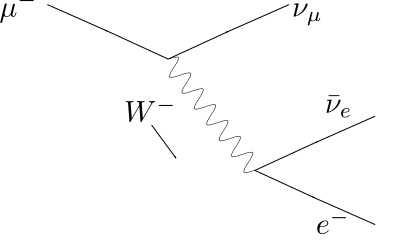
\includegraphics[scale=0.5]{muon_decay}
  \caption{diagrama de Feynman para el decaimiento $\mu^-\to \nu_\mu e^-\bar{\nu}_e$}
  \label{fig:muondecay}
\end{figure}
El propagador para el bosón $W$ de momentum $q$ resulta ser
\begin{align}
  \widetilde{D}_{\mu\nu}=\frac{1}{q^2-m_W^2}\left(g_{\mu\nu}-\frac{q_\mu q_\nu}{m_W^2}\right)\,.
\end{align}
Para los propósitos actuales la obtención de este resultado no es necesaria, el punto importante es que cuando los momentum de las partículas iniciales y finales son mucho más pequeñas que $m_W$, esto se reduce a
\begin{align}
  \widetilde{D}_{\mu\nu}=-\frac{g_{\mu\nu}}{m_W^2}\,.
\end{align}
Este resultado se entiende fácilmente cuando se compara con el propagador de una partículas escalar masiva $1/(q^2-M^2)\to-1/M^2$. Las componentes espaciales de $W_\mu$ con $\mu=1,2,3$, a bajas energías tienen el mismo propagador que el de una partícula escalar, mientras $W_0$, tiene el signo opuesto.

El Lagrangiano efectivo para el decaimiento del muón, $\mu^-\to \nu_\mu e^- \bar{\nu}_e$ es entonces
\begin{align}
  \mathcal{L}=&\frac{g^2}{8}\left[\bar{\nu}_\mu\gamma^\mu(1-\gamma_5)\mu\right]\frac{g_{\mu\nu}}{m_W^2}
  \left[\bar{e}\gamma^\nu(1-\gamma_5)\nu_e\right]\nonumber\\
=&\frac{g^2}{8m_W^2}\left[\bar{\nu}_\mu\gamma^\mu(1-\gamma_5)\mu\right]
  \left[\bar{e}\gamma^\nu(1-\gamma_5)\nu_e\right]\nonumber\\
  =&\frac{G_F}{\sqrt{2}}\left[\bar{\nu}_\mu\gamma^\mu(1-\gamma_5)\mu\right]\left[\bar{e}\gamma_\mu(1-\gamma_5)\nu_e\right]\,,
\end{align}
donde
\begin{align}
  \frac{G_F}{\sqrt{2}}=&\frac{g^2}{8m_W^2}\nonumber\\
  =&\frac{g^24}{8g^2v^2}\nonumber\\
  =&\frac{1}{2v^2}\,,
\end{align}
y
\begin{align}
  v=\left(\sqrt{2}G_F\right)^{-1/2}\,.
\end{align}


De otro lado, para el  decaimiento $\beta$, $n\to p e^- \bar{\nu}_e$, de acuerdo a la figura~\ref{fig:neutrondecay}, tenemos

\begin{align}
    \mathcal{L}=\frac{G_\beta}{\sqrt{2}}\left[\bar{p}\gamma^\mu(1-1.26\gamma_5)n\right]\left[\bar{e}\gamma_\mu(1-\gamma_5)\nu_e\right]\,.
\end{align}
\begin{figure}
  \centering
  \includegraphics[scale=0.5]{neutrondecay}
  \caption{Decaimiento del neutrón.}
  \label{fig:neutrondecay}
\end{figure}
con $G_F$ dado en la ec.~\eqref{eq:233qft} y $G_\beta=1.10\times 10^{-5}\,\text{GeV}^2$. La corriente hadrónica tiene la forma V--1.26A. El factor 1.26  puede entenderse como debido a las correcciones a nivel hadrónico de una corriente que es de la forma V--A a nivel del quarks, como en la ec.~\eqref{eq:234qft}. A nivel de quarks el decaimiento del neutrón ($udd$) al protón ($uud$) corresponde al decaimiento de uno de los quarks down del neutrón $d\to u e^- \bar{\nu}_e$
\begin{align}
    \mathcal{L}=\frac{G_F}{\sqrt{2}}V_{11}\left[\bar{u}\gamma^\mu(1-\gamma_5)d\right]\left[\bar{e}\gamma_\mu(1-\gamma_5)\nu_e\right]\,.
\end{align}
De modo que $G_\beta=G_F V_{11}=G_F\cos\theta_C$, donde $\theta_C$ es el ángulo de Cabbibo. Una vez se tienen en cuenta correcciones electrodébiles se obtiene el valor $|V_{11}|=0.97418(27)$\cite{PDG}. Las magnitudes de los elementos de la matriz CKM son\cite{PDG}
\begin{align}
  V\approx\begin{pmatrix}
    0.97419&0.2257&0.0359\\
    0.2256&0.97334&0.0415\\
    0.00874&0.0407&0.999133
  \end{pmatrix}\sim \mathbf{1}
\end{align}


\section{Apéndices}


\section{Interacci\'on Electrod\'ebil para leptones}
\label{sec:inter-electr}
El Lagrangiano de Dirac para la primera generaci\'on de leptones representados por los campos $\psi_e$ y $\psi_\nu$, es
\begin{align}
\mathcal{L}=i\overline{e_L}i\gamma^\mu\partial_\mu e_L+i\overline{e_R}i\gamma^\mu\partial_\mu e_R
  +i\overline{\nu_L}\gamma^\mu\partial_\mu\nu_L+i\overline{\nu_R}\gamma^\mu\partial_\mu\nu_R\nonumber\\
  -m_e(\overline{e_L}e_R+\overline{e_R}e_L)
  -m_\nu(\overline{\nu_L}\nu_R+\overline{\nu_R}\nu_L)
\end{align}
donde
\begin{equation}
  \psi_e\equiv e=e_L+e_R,\qquad \psi_\nu\equiv\nu_e=\nu_L+\nu_R\,.
\end{equation}
Este Lagrangiano debe dar cuenta de las caracter\'\i sticas de las interacciones d\'ebiles.
\subsection*{Corrientes V--A}
\label{sec:corrientes-v}
En dichas interacciones s\'olo participan las partes izquierdas de los campos. Esto nos permite prescindir del $\nu_R$, pues no tiene cargas d\'ebiles, fuertes o el\'ectricas
\begin{align}
  \label{eq:261}
  \mathcal{L}=i\overline{e_L}\gamma^\mu\partial_\mu e_L+i\overline{e_R}\gamma^\mu\partial_\mu e_R
  +i\overline{\nu_L}i\gamma^\mu\partial_\mu\nu_L-m_e(\overline{e_L}e_R+\overline{e_R}e_L)
\end{align}

\subsection*{Simetr\'\i a global $SU(2)_L\times U(1)_Y$}
\label{sec:simetr-glob-su2_l}

En el contexto de las interacciones d\'ebiles un $e_L$ es completamente equivalente a un campo $\nu_L$. Es decir, el Lagrangiano debe ser invariante bajo una transformaci\'on $SU(2)_L$ de esos campos. La diferencia entre ellos son sus respectivas cargas electricas y sus masas. Asumiendo que ambos campos tienen la misma hipercarga, podr\'\i amos esperar que la corriente electromagn\'etica apropiada puede obtenerse a partir del Grupo semisimple $SU(2)_L\times U(1)_Y$. Adem\'as las respectivas masas se podr\'\i an obtener a partir del mecanismo de Higgs. De hecho, definiendo el doblete 
  \begin{align}
    L\equiv\begin{pmatrix}
      \nu_L\\
      e_L      
    \end{pmatrix}\,,
  \end{align}
este transforma bajo $SU(2)_L$ como
\begin{align}
  L\to L'=&\exp(i T^i \theta_i)L\approx(1+i T^i\theta_i)L\nonumber\\
  \begin{pmatrix}
    \nu'_L\\
    e'_L
  \end{pmatrix}\approx&\begin{pmatrix}
    1+\frac{i}{2}&\frac{i}{2}\sqrt{2}\left(\frac{\theta_1-i\theta_2}{\sqrt{2}}\right)\\
    \frac{i}{2}\sqrt{2}\left(\frac{\theta_1+i\theta_2}{\sqrt{2}}\right)&1-i\frac{1}{2}
  \end{pmatrix}\begin{pmatrix}
    \nu_L\\
    e_L
  \end{pmatrix}\nonumber\\
  =&\begin{pmatrix}
    1+\frac{i}{2}&\frac{i}{2}\sqrt{2}\,\theta^+\\
    \frac{i}{2}\sqrt{2}\,\theta^-&1-i\frac{1}{2}
  \end{pmatrix}\begin{pmatrix}
    \nu_L\\
    e_L
  \end{pmatrix}\nonumber\\
  =&\begin{pmatrix}
    \left(1+\frac{i}{2}\right)\nu_L+\frac{i}{2}\sqrt{2}\,\theta^+e_L\\
    \left(1-\frac{i}{2}\right)e_L+\frac{i}{2}\sqrt{2}\,\theta^-\nu_L\\
  \end{pmatrix}\,.
\end{align}
Claramente el t\'ermino de masa $m_e$ en la ec.~(\ref{eq:261}) no es invariante bajo esta transformaci\'on. El Lagrangiano en la ec.~(\ref{eq:261}), sin t\'ermino de masa, puede reescribirse de manera que exhiba de forma m\'as explicita la invariante bajo $SU(2)_L$ como
\begin{align}
  \label{eq:219}
 \mathcal{L}=i\overline{L}\gamma^\mu\partial_\mu L+i\,\overline{e_R}\gamma^\mu\partial_\mu e_R\,,
\end{align}
donde, bajo $SU(2)_L$ $e_R$ transforma como
\begin{align}
  e_R\to e'_R=e_R\,.
\end{align}
Para que el Lagrangiano en la ec.~(\ref{eq:219}) sea invariante gauge global bajo $SU(2)_L\times U(1)_Y$, se debe satisfacer la relaci\'on de Gell--man--Nishijima \eqref{eq:184}
\begin{align}
  Q L=&
  \begin{pmatrix}
    0 \nu_L\\
    -1 e_L 
  \end{pmatrix}=
 (T_3+Y) L=
 \begin{pmatrix}
   \left(\frac{1}{2}+Y_L\right)\nu_L\\
   \left(-\frac{1}{2}+Y_L\right)e_L
 \end{pmatrix}
\nonumber\\
  Q e_R =&-1 e_R= Y\, e_R =Y_R\, e_R\,,
\end{align}
de modo que
\begin{align}
  Y_L&=-\frac{1}{2}& Y_R&=-1\,.
\end{align}
Concluimos que para que la simetr\'\i a gauge local bajo $SU(2)_L\times U(1)_Y$ sea exacta se requiere que la hipercarga $Y$ de ambas componentes del doblete sea la misma y que ambas tengan masa cero. Para tener un modelo consistente debe existir un mecanismo para generar la masa del electr\'on. 
\subsection*{Simetr\'\i a local $SU(2)_L\times U(1)_Y$}
\label{sec:simetr-local-su2_l}
Para que las cargas de isosp\'\i n d\'ebil se conserven localmente debemos cambiar la derivada normal en el Lagrangiano \eqref{eq:219} por la derivada covariante de $SU(2)_L\times U(1)_Y$
\begin{align}
  \label{eq:125}
  \partial^\mu\to\mathcal{D}^\mu&\equiv\partial^\mu-igT^iW^\mu_i-ig'YB^\mu\nonumber\\
&=  \begin{pmatrix}
    \partial^\mu-igT_3^\uparrow W^3_\mu-ig'YB_\mu&\frac{1}{\sqrt{2}}gW^+_\mu\\
    \frac{1}{\sqrt{2}}gW^-_\mu&\partial^\mu+igT_3^\downarrow W^3_\mu-ig'YB_\mu
  \end{pmatrix}.
\end{align}
y el Lagrangiano
\begin{align}
  \label{eq:220}
   \mathcal{L}=i\overline{L}\gamma^\mu\mathcal{D}_\mu L+i\,\overline{e_R}\gamma^\mu\mathcal{D}_\mu e_R
-\tfrac{1}{4}W^{\mu\nu}_i W_{\mu\nu}^i-\tfrac{1}{4}B^{\mu\nu} B_{\mu\nu}\,,
\end{align}
es el Lagrangiano invariante gauge local m\'as general posibles para los campos $e_{L,R}$, $\nu_L$, $W^\mu_i$, y $B^\mu$. De acuerdo a la ec.~\eqref{eq:124}
\begin{align}
  W^{\mu\nu}_i=\partial^\mu W^\nu_i -\partial^\nu W^\nu_i+g\,\epsilon^{ijk}W^\mu_j W^\nu_k.
\end{align}
Para escribir el Lagrangiano en una forma compacta, debemos introducir una convenci\'on: siempre que los t\'erminos de $\mathcal{D}^\mu$ act\'uen en un estado fermi\'onico de forma matricial diferente, el resultado es cero por definici\'on. As\'\i{} el resultado de hacer actuar $T^iW^\mu_i$ sobre el singlete bajo $SU(2)_L$, $e_R$, es cero. Note que
\begin{align}
  \mathcal{D}_\mu e_R=(\partial_\mu-ig' Y_R B_\mu)e_R\,.
\end{align}
En la secci\'on \ref{sec:invar-gauge-local-1} vimos que para tratar consistentemente el electromagnetismo conjuntamente con el grupo gauge local $SU(2)$, era necesario suponer inicialmente la existencia de un bos\'on gauge $B^\mu$ asociado a un grupo $U(1)_Y$ en lugar del $A^\mu$ electromagn\'etico asociado a $U(1)_Q$. El $A^\mu$ se puede obtener posteriormente a partir de una combinaci\'on lineal apropiada de $B^\mu$ y $W^\mu_3$, el bos\'on gauge diagonal de $SU(2)$. 

\subsection*{Mecanismo de Higgs}
\label{sec:mecanismo-de-higgs-1}
Como los bosones gauge $W^\mu_i$ deben ser masivos para dar cuenta de que la interacci\'on d\'ebil es de corto alcance, el Lagrangiano en ec.~\eqref{eq:220} debe ser complementado con un potencial escalar apropiado que pueda dar lugar a una ruptura espont\'anea de la simetr\'\i a. De acuerdo a la discusi\'on del Cap\'\i tulo \ref{rupt-espont-de} la escogencia m\'\i nima es introducir un doblete escalar complejo
\begin{equation}
  \Phi=
  \begin{pmatrix}
    \phi^+\\
    \phi^0
  \end{pmatrix}\,.
\end{equation} 
Entonces
\begin{align}
  \label{eq:221}
     \mathcal{L}=i\overline{L}\gamma^\mu\mathcal{D}_\mu L+i\,\overline{e_R}\gamma^\mu\mathcal{D}_\mu e_R
     -\tfrac{1}{4}W^{\mu\nu}_i W_{\mu\nu}^i-\tfrac{1}{4}B^{\mu\nu} B_{\mu\nu}
+(\mathcal{D}_\mu\Phi)^\dagger\mathcal{D}^\mu\Phi-\mu^2\Phi^\dagger\Phi-\lambda(\Phi^\dagger\Phi)^2\,,
\end{align}
donde $\mu^2\lt 0$, y $\lambda\gt 0$.



Los t\'erminos bos\'onicos en la ec.~(\ref{eq:221}), ya fueran analizados en la secci\'on \ref{sec:mecanismo-de-higgs},  eq.\eqref{eq:97}. 

\subsection*{Lagrangiano de Yukawa}
Para los campos del Lagrangiano en eq.~(\ref{eq:221}), debemos asegurarnos de que todos los t\'erminos invariantes gauge locales y renormalizables sean considerados. De hecho un t\'ermino de interacci\'on entre fermiones y el campo escalar, correspondiente a una interacci\'on de Yukawa, resulta ser invariante gauge local. Incluyendo dicho t\'ermino en el Lagrangiano invariante $SU(2)_L\times U(1)_Y$ para los campos $e$, $\nu_L$, $W_\mu^i$, $B_\mu$ y $\Phi$ tenemos
\begin{align}
  \label{eq:226}
     \mathcal{L}=&i\overline{L}\gamma^\mu\mathcal{D}_\mu L+i\,\overline{e_R}\gamma^\mu\mathcal{D}_\mu e_R\nonumber\\
     &-h_e\overline{L}\Phi e_R-h_e\overline{e_R}\Phi^\dagger L\nonumber\\
     &-\tfrac{1}{4}W^{\mu\nu}_i W_{\mu\nu}^i-\tfrac{1}{4}B^{\mu\nu} B_{\mu\nu}\nonumber\\
     &+(\mathcal{D}_\mu\Phi)^\dagger\mathcal{D}^\mu\Phi-\mu^2\Phi^\dagger\Phi+\lambda(\Phi^\dagger\Phi)^2\,.
\end{align}
Bajo una transformaci\'on gauge local los campos transforman como:
\begin{align}
  \mathcal{D}_\mu L&\to\left(\mathcal{D}_\mu L\right)'=\exp\left(-iT^i\theta_i-iY_L\right)\mathcal{D}_\mu L\nonumber\\
  \mathcal{D}_\mu e_R&\to\left(\mathcal{D}_\mu e_R\right)'=\exp\left(-iY_R\right)\mathcal{D}_\mu e_R\nonumber\\
  \Phi&\to\Phi'=\exp\left(-iT^i\theta_i-iY_\Phi\right)\Phi,
\end{align}
Y la acci\'on determinada por el Lagrangiano en ec.~\eqref{eq:226} permanece invariante bajo $SU(2)_L\times U(1)_Y$. Parte de los t\'erminos del Lagrangiano ya han sido analizados en el Cap\'\i tulo \ref{rupt-espont-de}. 

\subsection*{Gauge Unitario}
Para obtener el espectro despu\'es de la ruptura espont\'anea de simetr\'\i a es conveniente usar el Gauge Unitario para reescribir el campo de Higgs como en la ec.~\eqref{eq:123}
\begin{equation}
      \Phi=
  \begin{pmatrix}
    0\\
    \frac{1}{\sqrt{2}}[H(x)+v]
  \end{pmatrix}\,.
\end{equation}
Usando los resultados de la secci\'on \ref{sec:mecanismo-de-higgs} tenemos
\begin{align}
  \mathcal{L}_{H W B}=&\left(\mathcal{D}^\mu\Phi\right)^\dagger\mathcal{D}_\mu\Phi-\mu^2\Phi^\dagger \Phi-\lambda\left(\Phi^\dagger\Phi\right)^2\nonumber\\
  =&\frac{1}{2}\partial^\mu H\partial_\mu H-V(H)\nonumber\\
&+\frac{1}{4}g^2{W^\mu}^-W_\mu^+H^2+\frac{1}{2}vg^2{W^\mu}^-W_\mu^+H\nonumber\\
  &+\frac{1}{2}\left(\frac{g}{2\cos\theta_W}\right)^2Z^\mu Z_\mu H^2+\left(\frac{g}{2\cos\theta_W}\right)^2v\,Z^\mu Z_\mu H\nonumber\\
  &+\frac{1}{2}m_W^2{W^\mu}^-W_\mu^++\frac{1}{2}m_W^2{W^\mu}^-W_\mu^+ +\frac{1}{2}m_Z^2Z^\mu Z_\mu\,,
\end{align}
donde:
%instiki:
\begin{itemize} %noinstiki
\item
  \begin{align}
    V(H)=&\tfrac{1}{2}m_H^2H^2+\lambda vH^3+\tfrac{1}{4}\lambda H^4\nonumber\\
    =&\frac{1}{2}m_H^2H^2+\frac{m_H^2}{2v}H^3+\frac{1}{4}\frac{m_H^2}{2v^2} H^4\nonumber\\
    =&\frac{1}{2}m_H^2H^2\left(1+\frac{H}{v}+\frac{H^2}{4v^2}\right)\,.
  \end{align}
con
\begin{equation}
  m_H^2=-2\mu^2=2\lambda v^2.
\end{equation}

\item 
\begin{equation}
\label{eq:262}
  \begin{pmatrix}
    W^3_\mu\\
    B_\mu
  \end{pmatrix}=\begin{pmatrix}
    \cos\theta_W & \sin\theta_W\\
    -\sin\theta_W& \cos\theta_W
  \end{pmatrix}
  \begin{pmatrix}
    Z_\mu\\
    A_\mu
  \end{pmatrix},
\end{equation}
tal que
\begin{equation}
  \label{eq:263}
  g\sin\theta_W=g'\cos\theta_W=e.
\end{equation}
\item
  \begin{equation}
    m_W=\frac{gv}{2}\qquad m_Z=\frac{m_W}{\cos\theta_W}.
  \end{equation}
\end{itemize} %noinstiki
%instiki:
Entonces
\begin{align}
\mathcal{L}_{H W B}=&\frac{1}{2}\partial^\mu H\partial_\mu H-V(H)\nonumber\\
&+m_W^2{W^\mu}^-W_\mu^++\frac{g^2v^2}{4v^2}(2vH+H^2){W^\mu}^-W_\mu^+\nonumber\\
  &+\frac{1}{2}m_Z^2Z^\mu Z_\mu+\frac{1}{2v^2}\left(\frac{gv}{2\cos\theta_W}\right)^2(2vH+H^2)Z^\mu Z_\mu\nonumber\\
  =&\frac{1}{2}\partial^\mu H\partial_\mu H-V(H)
  +m_W^2\left(1+2\frac{H}{v}+\frac{H^2}{v^2}\right){W^\mu}^-W_\mu^+
  +\frac{1}{2}m_Z^2\left(1+2\frac{H}{v}+\frac{H^2}{v^2}\right)Z^\mu Z_\mu\,.
\end{align}
Adem\'as
\begin{align}
  \mathcal{L}_{l W B}=&i\overline{L}\gamma^\mu\mathcal{D}_\mu L+i\,\overline{e_R}\gamma^\mu\mathcal{D}_\mu e_R
\end{align}
Donde, usando el mismo procedimiento se obtiene el resultado an\'alogo para la ec.~\eqref{eq:187}
\begin{align}
 \mathcal{L}_{l W B}=i\overline{L}\gamma^\mu[\partial_\mu-i g (T^1W_\mu^1+T^2W_\mu^2)-i(g T^3W_\mu^3+g' Y B_\mu)]L
+i\overline{e_R}\gamma^\mu(\partial_\mu-i g' Y B_\mu)e_R
\end{align}
Ya que
\begin{align}
  T^1W_\mu^1+T^2W_\mu^2=&\frac{1}{2}
  \begin{pmatrix}
    0             &W_\mu^1-i W_\mu^2\\
    W_\mu^1-i W_\mu^2  & 0          \\
  \end{pmatrix}=\frac{\sqrt{2}}{2}
  \begin{pmatrix}
    0             &W_\mu^+\\
    W_\mu^-  & 0          \\
  \end{pmatrix}
\end{align}
\begin{align}
\mathcal{L}_{l W B}=&i\overline{\nu_L}\gamma^\mu\partial_\mu\nu_L+i\overline{e_L}\gamma^\mu\partial_\mu e_L
+i\overline{e_R}\gamma^\mu\partial_\mu e_R+
  \frac{g}{\sqrt{2}}\begin{pmatrix}
    \overline{\nu_L}&\overline{e_L}
  \end{pmatrix} 
  \begin{pmatrix}
    0             &W_\mu^+\\
    W_\mu^-  & 0          \\
  \end{pmatrix}
  \begin{pmatrix}
    \nu_L\\
    e_L
  \end{pmatrix}\nonumber\\
&+\overline{L}\gamma^\mu\left(\frac{g}{2}\tau_3W_\mu^3+g'Y B_\mu\right)L+
g'\overline{e_R}\gamma^\mu Y_R B_\mu e_R
\end{align}
usando ec.~\eqref{eq:262}
\begin{align}
  \mathcal{L}_{l W B}=&i\overline{\nu_L}\gamma^\mu\partial_\mu\nu_L+i\overline{e}\gamma^\mu\partial_\mu e
+\frac{g}{\sqrt{2}}\left(\overline{e_L}W_\mu^-\nu_L+\overline{\nu_L}W_\mu^+e_L\right)+\nonumber\\
&\overline{L}\gamma^\mu\left[\frac{g}{2}\tau_3(c_W Z_\mu+s_W A_\mu)
+g'Y(-s_W Z_\mu+c_W A_\mu)\right]L+\nonumber\\
&g'\overline{e_R}\gamma^\mu Y_R(-s_W Z_\mu+c_W A_\mu) e_R\nonumber\\
=&i\overline{\nu_L}\gamma^\mu\partial_\mu\nu_L+i\overline{e}\gamma^\mu\partial_\mu e
+\frac{g}{\sqrt{2}}\left(\overline{e_L}W_\mu^-\nu_L+\overline{\nu_L}W_\mu^+e_L\right)+\nonumber\\
&\overline{L}\gamma^\mu\left[\left(\frac{g c_W}{2}\tau_3 -g's_W Y \right)Z_\mu
+\left(\frac{g s_W}{2}\tau_3 +g'c_W Y \right)A_\mu\right]L\nonumber\\
&-g's_W\overline{e_R}\gamma^\mu Y_R Z_\mu e_R+g'c_W\overline{e_R}\gamma^\mu Y_R A_\mu e_R
\end{align}
usando ec.~(\ref{eq:263})

\begin{align}
\mathcal{L}_{l W B}=&i\overline{\nu_L}\gamma^\mu\partial_\mu\nu_L+i\overline{e}\gamma^\mu\partial_\mu e
+\frac{g}{\sqrt{2}}\left(\overline{e_L}W_\mu^-\nu_L+\overline{\nu_L}W_\mu^+e_L\right)+\nonumber\\
&\overline{L}\gamma^\mu\left(\frac{g c_W}{2}\tau_3 -g\frac{s^2_W}{c_W} Y \right)L Z_\mu
+e\overline{L}\gamma^\mu\left(\frac{\tau_3}{2} + Y \right) L A_\mu\nonumber\\
&-g \frac{s^2_W}{c_W}\overline{e_R}Y_R e_R Z_\mu+e \overline{e_R}Y_R e_R A_\mu\nonumber\\
=&i\overline{\nu_L}\gamma^\mu\partial_\mu\nu_L+i\overline{e}\gamma^\mu\partial_\mu e
+\frac{g}{\sqrt{2}}\left(\overline{e_L}W_\mu^-\nu_L+\overline{\nu_L}W_\mu^+e_L\right)+\nonumber\\
&\frac{g}{c_W}\overline{L}\gamma^\mu\left( c^2_W\frac{\tau_3}{2} - s^2_W Y \right)L Z_\mu
+e\overline{L}\gamma^\mu Q L A_\mu\nonumber\\
&-g \frac{s^2_W}{c_W}\overline{e_R}\gamma^\mu Y_R e_R Z_\mu+e \overline{e_R}\gamma^\mu Q_e e_R A_\mu\nonumber\\
=&i\overline{\nu_L}\gamma^\mu\partial_\mu\nu_L+i\overline{e}\gamma^\mu\partial_\mu e
+\frac{g}{\sqrt{2}}\left(\overline{e_L}W_\mu^-\nu_L+\overline{\nu_L}W_\mu^+e_L\right)+\nonumber\\
&+e\overline{e_L}\gamma^\mu Q_e e_L A_\mu+e \overline{e_R}Q_e e_R A_\mu\nonumber\\
&+\frac{e}{s_W c_W}\overline{L}\gamma^\mu\left[ (1-s^2_W)\frac{\tau_3}{2} -s^2_WY \right]L Z_\mu
-\frac{e}{s_W c_W}\overline{e_R}\gamma^\mu s^2_W Y_R e_R Z_\mu\nonumber\\
=&i\overline{\nu_L}\gamma^\mu\partial_\mu\nu_L+i\overline{e}\gamma^\mu\partial_\mu e
+\frac{g}{\sqrt{2}}\left(\overline{e_L}W_\mu^-\nu_L+\overline{\nu_L}W_\mu^+e_L\right)\nonumber\\
&+e\overline{e}P_R\gamma^\mu Q_e P_L e A_\mu+e \overline{e}P_L Q_e P_R e A_\mu\nonumber\\
&+\frac{e}{s_W c_W}\overline{L}\gamma^\mu\left[ \frac{\tau_3}{2}-s^2_W Q \right]L Z_\mu
-\frac{e}{s_W c_W}\overline{e_R}\gamma^\mu s^2_W Y_R e_R Z_\mu\nonumber\\
=&i\overline{\nu_L}\gamma^\mu\partial_\mu\nu_L+i\overline{e}\gamma^\mu\partial_\mu e
+\frac{g}{\sqrt{2}}\left(\overline{e_L}W_\mu^-\nu_L+\overline{\nu_L}W_\mu^+e_L\right)\nonumber\\
&+e\overline{e}\gamma^\mu Q_e e A_\mu\nonumber\\
&+\frac{e}{2s_W c_W}\overline{L}\gamma^\mu\left[\tau_3-2Q s^2_W\right]L Z_\mu
-\frac{e}{2s_W c_W}\overline{e_R}\gamma^\mu2s^2_W Q_e e_R Z_\mu
\end{align}
De modo que
\begin{align}
\mathcal{L}_{l W B}=i\bar{e}\gamma^\mu\partial_\mu e+i\bar{\nu_e}\gamma^\mu\partial_\mu\nu_e+\mathcal{L}_{cc}+\mathcal{L}_{nc}
\end{align}
donde
\begin{align}
\label{eq:228}
\mathcal{L}_{nc}=&eJ^\mu_{\text{EM}}A_\mu+\frac{e}{2\cos\theta_W\sin\theta_W}J^\mu_{\text{NC}}Z_\mu
\end{align}
donde ahora
\begin{align}
  J^\mu_{\text{EM}}=\bar{e}\gamma^\mu Q e=-\bar{e}\gamma^\mu e
\end{align}
y 
\begin{align}
  J^\mu_{\text{NC}}=\sum_{\Psi=L,e_R}\overline{\Psi}\gamma^\mu\left(\tau^3-2Q\sin^2\theta_W\right)\Psi\,.
\end{align}
En t\'erminos de los ferminones usuales
\begin{align}
   J^\mu_{\text{NC}}=&\overline{L}\gamma^\mu\left[\tau_3-2Q s^2_W\right]L 
-\frac{e}{2s_W c_W}\overline{e_R}\gamma^\mu2s_W^2Q_e e_R \nonumber\\
  =&\begin{pmatrix}
  \overline{\nu_L} & \overline{e_L}  
  \end{pmatrix}
\gamma^\mu
\begin{pmatrix}
  1 & 0\\
  0           & -1+2s_W^2
\end{pmatrix}
\begin{pmatrix}
  \nu_L\\
  e_L
\end{pmatrix}
 +\overline{e_R}\gamma^\mu2s_W^2 e_R \nonumber\\
   =&\overline{\nu}\gamma^\mu P_L\nu
+\overline{e}\gamma^\mu\left(-1+2s^2_W\right)P_L e
+\overline{e}\gamma^\mu2s_W^2P_R e\nonumber\\
   =&\overline{\nu}\gamma^\mu\left(\frac{1}{2}-\frac{\gamma_5}{2}\right)\nu
+\overline{e}\gamma^\mu\left(-1+2s^2_W\right)\frac{(1-\gamma_5)}{2} e
+\overline{e}\gamma^\mu2s_W^2\frac{(1+\gamma_5)}{2}e\nonumber\\
   =&\overline{\nu}\gamma^\mu\left(\frac{1}{2}-\frac{\gamma_5}{2}\right)\nu
+\overline{e}\gamma^\mu\left(-\frac{1}{2}+2s^2_W+\frac{1}{2}\gamma_5\right) e
\end{align}
%\left(\right)
\begin{align}
  J^\mu_{NC}=\sum_{f=e,\nu_e}\bar{f}\gamma^\mu(v_f-a_f\gamma_5)f\,,
\end{align}
donde $2v_e=-1+4\sin^2\theta_W$, $2a_e=-1$, $v_{\nu_e}=a_{\nu_e}=1$. 

Igual que en el caso de $SU(3)_C$
\begin{align}
  \mathcal{L}_{cc}=
  =&\frac{g}{\sqrt{2}}\left[\overline{e_L}\gamma^\mu\nu_L W_\mu^-+\overline{\nu_L}\gamma^\mu e_L W_\mu^+\right]\nonumber\\
  =&\frac{g}{2\sqrt{2}}\left[\bar{e}\gamma^\mu(1-\gamma_5)\nu_e W_\mu^-+\bar{\nu}_e\gamma^\mu(1-\gamma_5)e W_\mu^+\right]
\end{align}
Para el t\'ermino de Yukawa
\begin{align}
  \mathcal{L}_{fH}=&h_e \left(\overline{L}\Phi e_R+\overline{e_R}\Phi^\dagger L\right)\nonumber\\
  =&\frac{h_e}{\sqrt{2}} \left(\overline{e_L}e_R+\overline{e_R}e_R\right)(H+v)\nonumber\\
  =&m_e\overline{e}e+\frac{h_e}{\sqrt{2}}\overline{e}e H\nonumber\\
  =&m_e\overline{e}e+{m_e}\overline{e}e \frac{H}{v}\nonumber\\
  =&m_e\overline{e}e\left(1+\frac{H}{v}\right) \,.
\end{align}
donde
\begin{equation}
  m_e=\frac{h_e v}{\sqrt{2}}\,.
\end{equation}

De modo que el mismo mecanismo que da cuenta de la masa de los bosones gauge, da cuenta de la masa de los fermiones y entrega una interacci\'on con la que se puede comprobar experimentalmente el modelo. Encontrar estas interacciones del Higgs con los fermiones y con los bosones gauge es el principal objetivo del LHC. 

Como se vi\'o en la secci\'on \ref{sec:mecanismo-de-higgs} los t\'erminos cin\'eticos de los bosones gauge se pueden escribir en t\'erminos de $W^\pm$ $Z_\mu$ y $A_\mu$, 
\begin{align}
  \mathcal{L}_{W B}=&-\tfrac{1}{4}W^{\mu\nu}_i W_{\mu\nu}^i-\tfrac{1}{4}B^{\mu\nu} B_{\mu\nu}\nonumber\\
  =&-\tfrac{1}{4}F^{\mu\nu} F_{\mu\nu}-\tfrac{1}{4}Z^{\mu\nu} Z_{\mu\nu}-\tfrac{1}{2}(F_W^\dagger)^{\mu\nu} (F_W)_{\mu\nu}-\mathcal{L}_3-\mathcal{L}_4
\end{align}
donde
\begin{equation}
  (F_W)_{\mu\nu}=\partial_\mu W^+_\nu-\partial_\nu W^+_\mu
\end{equation}
y $\mathcal{L}_3$ y $\mathcal{L}_4$ est\'an dados en \cite{Pich:2005mk}
\begin{align}
  \mathcal{L}_3=&-ie\cot\theta_W\left[(F_W^\dagger)^{\mu\nu}W_\mu^+ Z_\nu-(F_W)^{\mu\nu}W_\mu^- Z_\nu+W_\mu^-W_\nu^+Z^{\mu\nu}\right]\nonumber\\
&-ie\left[(F_W^\dagger)^{\mu\nu}W_\mu^+ A_\nu-(F_W)^{\mu\nu}W_\mu^- A_\nu+W_\mu^-W_\nu^+F^{\mu\nu}\right]\,,
\end{align}
\begin{align}
\mathcal{L}_4=  &-\frac{e^2}{2\sin^2\theta_W}\left[\left(W_\mu^+{W^\mu}^-\right)^2-W_\mu^+{W^\mu}^+W_\nu^-{W^\nu}^-\right]
-e^2\cot^2\theta_W\left(W_\mu^+{W^\mu}^-Z_\nu Z^\nu-W_\mu^+Z^\mu W_\nu^-Z^\nu\right)\nonumber\\
&-e^2\cot^2\theta_W\left(2W_\mu^+{W^\mu}^-A_\nu Z^\nu-W_\mu^+A^\mu W_\nu^-Z^\nu-W_\mu^+Z^\mu W_\nu^-A^\nu\right)\nonumber\\
&-e^2\left(W_\mu^+{W^\mu}^-A_\nu A^\nu-W_\mu^+A^\mu W_\nu^-A^\nu\right)\,.
\end{align}

%\left(\right)
En resumen el Lagrangiano invariante gauge local bajo $SU(2)_L\times U(1)_Y$ dado en la ec.~(\ref{eq:226}), escrito en el gauge unitario es ($f=e,\nu_e$, y tal que para $f=\nu_e$, $f'=e$)
\begin{align}
\mathcal{L}_{\text{EW}}=&\sum_f i\bar{f}\left(\gamma^\mu\partial_\mu-m_f\right)f
-\tfrac{1}{4}F^{\mu\nu} F_{\mu\nu}-\tfrac{1}{4}Z^{\mu\nu} Z_{\mu\nu}-\tfrac{1}{2}(F_W^\dagger)^{\mu\nu} (F_W)_{\mu\nu}
+\tfrac{1}{2}\partial^\mu H\partial_\mu H\nonumber\\
&-\frac{1}{2}m_H^2H^2\left(1+\frac{H}{v}+\frac{H^2}{4v^2}\right)
+\left(m_W^2{W^\mu}^-W_\mu^++\frac{1}{2}m_Z^2Z^\mu Z_\mu\right)\left(1+2\frac{H}{v}+\frac{H^2}{v^2}\right)\nonumber\\
&+e\sum_f \bar{f}\gamma^\mu Q_f f A_\mu+\frac{e}{2\cos\theta_W\sin\theta_W}\sum_{f}\bar{f}\gamma^\mu(v_f-a_f\gamma_5)f Z_\mu\nonumber\\
&+\frac{g}{2\sqrt{2}}\left[\sum_{f=\nu_e}\bar{f}\gamma^\mu(1-\gamma_5)f' W_\mu^++\text{h.c}\right]
+\sum_f \frac{m_f}{v} \bar{f}f H\nonumber\\
&-ie\cot\theta_W\left[(F_W^\dagger)^{\mu\nu}W_\mu^+ Z_\nu-(F_W)^{\mu\nu}W_\mu^- Z_\nu+W_\mu^-W_\nu^+Z^{\mu\nu}\right]\nonumber\\
&-ie\left[(F_W^\dagger)^{\mu\nu}W_\mu^+ A_\nu-(F_W)^{\mu\nu}W_\mu^- A_\nu+W_\mu^-W_\nu^+F^{\mu\nu}\right]\nonumber\\
&-\frac{e^2}{2\sin^2\theta_W}\left[\left(W_\mu^+{W^\mu}^-\right)^2-W_\mu^+{W^\mu}^+W_\nu^-{W^\nu}^-\right]
-e^2\cot^2\theta_W\left(W_\mu^+{W^\mu}^-Z_\nu Z^\nu-W_\mu^+Z^\mu W_\nu^-Z^\nu\right)\nonumber\\
&-e^2\cot^2\theta_W\left(2W_\mu^+{W^\mu}^-A_\nu Z^\nu-W_\mu^+A^\mu W_\nu^-Z^\nu-W_\mu^+Z^\mu W_\nu^-A^\nu\right)\nonumber\\
&-e^2\left(W_\mu^+{W^\mu}^-A_\nu A^\nu-W_\mu^+A^\mu W_\nu^-A^\nu\right)\,.
\end{align}
donde $m_{\nu_e}=0$.

\subsection{Dispersi\'on electron--neutrino}
\label{sec:disp-electr-neutr}
Comparando con el Lagrangiano efectivo de la dispersi\'on $\nu_e + e^- \to \nu_e + e^-$ se obtiene
\begin{align}
  v=\left(\sqrt{2}\,G_F\right)^{-1/2}=246.2\,\text{GeV}\,.
\end{align}


\section{Modelo Est\'andar}
\label{sec:modelo-estandar-1}

\subsection{Primera generaci\'on}
\label{sec:una-generacion}
Introduciendo los quarks $u$ y $d$, tenemos como contenido de part\'\i culas
\begin{align}
  L=&\begin{pmatrix}
    \nu_L\\
    e_L
  \end{pmatrix},\qquad e_R\nonumber\\
  Q^\alpha=&\begin{pmatrix}
    u_L^\alpha\\
    d_L^\alpha
  \end{pmatrix},\qquad u_R^a,\quad d_R^\alpha
\end{align}
donde $\alpha$ es el \'\i ndice de color. Productos del tipo $\overline{u_L}^\alpha u_L^\alpha$ ser\'an denotados simplemente como $\overline{u_L}u_L$. Adem\'as 
\begin{align}
  \nu_L=&P_L\nu_e,& e_{L,R}=&P_{L,R}\,e\nonumber\\
  u_{L,R}=&P_{L,R}\,u,& d_{L,R}=&P_{L,R}\,d\,.
\end{align}
Como antes, el t\'ermino $\overline{Q}\Phi$ es invariante bajo $SU(2)_L$. Hemos mostrado en problema \ref{cha:princ-gauge-local}.\ref{item:pch3.3}. que si
$\overline{Q}\Phi$ es un invariante $SU(2)$, el t\'ermino ${\tilde \Phi}^\dagger Q$ tambi\'en es un invariante de $SU(2)$. Expl\'\i citamente
\begin{align}
  \widetilde{\Phi}^\dagger Q=&(i\tau_2\Phi^*)^\dagger Q\nonumber\\
  =& \begin{pmatrix}
    {\phi^0}^*\\
    -\phi^-    
  \end{pmatrix}^\dagger Q\nonumber\\
  =&\begin{pmatrix}
    \phi^0 & -\phi^+
  \end{pmatrix}\begin{pmatrix}
    u_L\\
    d_L
  \end{pmatrix}\nonumber\\
  =&\phi^0 u_L - \phi^+ d_L\nonumber\\
  =&\epsilon_{12}Q_1\Phi_2+\epsilon_{21}Q_2\Phi_1\nonumber\\
  =&\epsilon_{ab}Q_a \Phi_b\,.
\end{align}
Bajo una transformaci\'on $SU(2)_L$
\begin{align}
\widetilde{\Phi}^\dagger Q\to {\widetilde{\Phi'}}^\dagger Q'=\epsilon_{ab}Q'_a \Phi'_b=&\epsilon_{ab}U_{ac}U_{bd}Q_c \Phi_d\nonumber\\
  =&\epsilon_{cd}\det\mathbf{U} Q_c \Phi_d\nonumber\\
  =&\epsilon_{cd} Q_c \Phi_d\nonumber\\
  =&\widetilde{\Phi}^\dagger Q\,.
\end{align}
Las hipercargas se obtienen de
\begin{align}
  \begin{pmatrix}
    \frac{2}{3}u_L\\
    -\frac{1}{3}d_L
  \end{pmatrix}=&
  (T_3+Y_Q)
  \begin{pmatrix}
    u_L\\
    d_L
  \end{pmatrix}=
  \begin{pmatrix}
    (\frac{1}{2}+Y_Q)u_L\\
    (-\frac{1}{2}+Y_Q)d_L
  \end{pmatrix}\nonumber\\
  \begin{pmatrix}
    0\times{\phi^0}^*\\
    -(-\phi^-)
  \end{pmatrix}=&
  (T_3+Y_Q)
  \begin{pmatrix}
    {\phi^0}^*\\
    -\phi^-
  \end{pmatrix}=
  \begin{pmatrix}
    (\frac{1}{2}+Y_{\widetilde{\Phi}}){\phi^0}^*\\
    (-\frac{1}{2}+Y_{\widetilde{\Phi}})(-\phi^-)
  \end{pmatrix}
\end{align}
Entonces
\begin{equation}
  Y_Q=\frac{2}{3}-\frac{1}{2}=1/6,\quad Y_{\widetilde{\Phi}}=-\frac{1}{2},\quad Y_{u_R}=\frac{2}{3}
,\quad Y_{d_R}=-\frac{1}{3}\,.
\end{equation}
Bajo hipercarga
\begin{align}
\overline{Q}\Phi\to&e^{i(1/3)\alpha}\overline{Q}\Phi\nonumber\\
\widetilde{\Phi}^\dagger Q\to&e^{i(2/3)\alpha}\widetilde{\Phi}^\dagger Q\,
\end{align}
Entonces podemos construir los invariantes bajo $SU(3)_c\times SU(2)_L\times U(1)_Y$ como
\begin{align}
  \mathcal{L}_{\text{Yukawa}}=&h_d\overline{Q}\Phi d_R+h_u\overline{u_R}\widetilde{\Phi}^\dagger Q+\text{h.c}\nonumber\\
  =&h_d\overline{Q}\Phi d_R+h_u\overline{u_R}\widetilde{\Phi}^\dagger Q+h_d\overline{d_R}\Phi^\dagger Q+h_u\overline{Q}\widetilde{\Phi}u_R\nonumber\\
=&h_d\overline{Q}\Phi d_R+h_u\overline{Q}\widetilde{\Phi}u_R+\text{h.c}\,
\end{align}
Recuerde que $\overline{Q}\Phi d_R=\overline{Q}_\alpha\Phi d_R^\alpha$.
El Lagrangiano invariante gauge local bajo $SU(3)_c\times SU(2)_L\times U(1)_Y$ es entonces
\begin{align}
     \mathcal{L}=&i\sum_{\Psi=L,e_R,Q,u_R,d_R}\overline{\Psi}\gamma^\mu\mathcal{D}_\mu \Psi\nonumber\\
     &-(h_e\overline{L}\Phi e_R+h_d\overline{Q}\Phi d_R+h_u\overline{Q}\widetilde{\Phi}u_R+\text{h.c})\nonumber\\
     &-\tfrac{1}{4}W^{\mu\nu}_i W_{\mu\nu}^i-\tfrac{1}{4}B^{\mu\nu} B_{\mu\nu}\nonumber\\
     &+(\mathcal{D}_\mu\Phi)^\dagger\mathcal{D}^\mu\Phi-\mu^2\Phi^\dagger\Phi+\lambda(\Phi^\dagger\Phi)^2\,.
\end{align}
Donde
\begin{align}
  \mathcal{D}^\mu&\equiv\partial^\mu-i g_s\frac{\lambda^a}{2}G^\mu_a-i g \frac{\tau^i}{2}W^\mu_i-i g'YB^\mu\,.
\end{align}
En el gauge unitario
\begin{align}
  \Phi=&\begin{pmatrix}
    0\\
    \frac{1}{\sqrt{2}}(H(x)+v)
  \end{pmatrix}&  \widetilde{\Phi}=&\begin{pmatrix}
    \frac{1}{\sqrt{2}}(H(x)+v)\\
    0
  \end{pmatrix}\,,
\end{align}
y utilizando los resultados para la Cromodin\'amica Cu\'antica de la secci\'on~\ref{sec:inter-fuert}, el Lagrangiano para $f=\nu_e,e,u,d$, $q=u,d$ y $f'=e$ ($d$) para $f=\nu_e$ ($u$) es
\begin{align}
  \mathcal{L}_{\text{1 gen}}=&\sum_f i\bar{f}\left(\gamma^\mu\partial_\mu-m_f\right)f
-\tfrac{1}{4}F^{\mu\nu} F_{\mu\nu}-\tfrac{1}{4}Z^{\mu\nu} Z_{\mu\nu}-\tfrac{1}{2}(F_W^\dagger)^{\mu\nu} (F_W)_{\mu\nu}
- \tfrac{1}{4}\widetilde{G}^{\mu\nu}_a \widetilde{G}_{\mu\nu}^a\nonumber\\
&+\tfrac{1}{2}\partial^\mu H\partial_\mu H
-\frac{1}{2}m_H^2H^2\left(1+\frac{H}{v}+\frac{H^2}{4v^2}\right)
+\left(m_W^2{W^\mu}^-W_\mu^++\frac{1}{2}m_Z^2Z^\mu Z_\mu\right)\left(1+2\frac{H}{v}+\frac{H^2}{v^2}\right)\nonumber\\
&+g_s\sum_q\bar{q}\gamma^\mu\left(\frac{\lambda_a}{2}\right)q\,G_\mu^a+e\sum_f \bar{f}\gamma^\mu Q_f f A_\mu+\frac{e}{2\cos\theta_W\sin\theta_W}\sum_{f}\bar{f}\gamma^\mu(v_f-a_f\gamma_5)f Z_\mu\nonumber\\
&+\frac{g}{2\sqrt{2}}\left[\sum_{f}\bar{f}\gamma^\mu(1-\gamma_5)f' W_\mu^++\text{h.c}\right]
+\sum_f \frac{m_f}{v} \bar{f}f H\nonumber\\
&-ie\cot\theta_W\left[(F_W^\dagger)^{\mu\nu}W_\mu^+ Z_\nu-(F_W)^{\mu\nu}W_\mu^- Z_\nu+W_\mu^-W_\nu^+Z^{\mu\nu}\right]\nonumber\\
&-ie\left[(F_W^\dagger)^{\mu\nu}W_\mu^+ A_\nu-(F_W)^{\mu\nu}W_\mu^- A_\nu+W_\mu^-W_\nu^+F^{\mu\nu}\right]\nonumber\\
&-\frac{e^2}{2\sin^2\theta_W}\left[\left(W_\mu^+{W^\mu}^-\right)^2-W_\mu^+{W^\mu}^+W_\nu^-{W^\nu}^-\right]
-e^2\cot^2\theta_W\left(W_\mu^+{W^\mu}^-Z_\nu Z^\nu-W_\mu^+Z^\mu W_\nu^-Z^\nu\right)\nonumber\\
&-e^2\cot^2\theta_W\left(2W_\mu^+{W^\mu}^-A_\nu Z^\nu-W_\mu^+A^\mu W_\nu^-Z^\nu-W_\mu^+Z^\mu W_\nu^-A^\nu\right)\nonumber\\
&-e^2\left(W_\mu^+{W^\mu}^-A_\nu A^\nu-W_\mu^+A^\mu W_\nu^-A^\nu\right)\nonumber\\
&- \frac{1}{4}\left(g_s\widetilde{G}^{\mu\nu}_af_{a d e}G^d_\mu G^e_\nu
    +g_sf^{a b c}G_b^\mu G_c^\nu\widetilde{G}_{\mu\nu}^a
    +g_s^2f^{a b c}f_{a d e}G_b^\mu G_c^\nu G^d_\mu G^e_\nu\right)\,.
\end{align}
donde
\begin{equation}
  \widetilde{G}^{\mu\nu}=\partial^\mu G^\nu_a-\partial^\nu G^\mu
\end{equation}
En la tabla~\ref{tab:zcoup} se muestran los acoplamientos de las corrientes neutras.
%noinstiki
\begin{table}  %noinstiki
  \centering %noinstiki
  \begin{tabular}{l|c|c|c|c} %noinstiki
   $f=$ &$u$&$d$&$\nu_e$&$e$\\\hline{}
$2v_f$&$1-\frac{8}{3}\sin^2\theta_W$&$-1+\frac{4}{3}\sin^2\theta_W$&$1$&$-1+4\sin^2\theta_W$\\
$2a_f$&$1$&$-1$&$1$&$-1$\\
  \end{tabular} %noinstiki
  \caption{Acoplamientos de corrientes neutras} %noinstiki
\label{tab:zcoup}
\end{table} %noinstiki
%noinstiki

\subsection{Din\'amica de sabor}
\label{sec:dinamica-de-sabor}
El Modelo Est\'andar esta compuesto de las siguientes tres familias de fermiones $i=1,2,3$. A cada familia se le asigna una carga de \emph{sabor} diferente
\begin{align}
L_i=&
\begin{pmatrix}
  \nu^i_L\\
  e^i_L
\end{pmatrix}:&
  L_1=&
  \begin{pmatrix}
    \nu^e_L\\
    e_L
  \end{pmatrix}&  L_2=&
  \begin{pmatrix}
    \nu^\mu_L\\
    \mu_L
  \end{pmatrix}&  L_3=&
  \begin{pmatrix}
    \nu^\tau_L\\
    \tau_L
  \end{pmatrix}& e_R^i:\;e_R,\;\mu_R,\;\tau_R\nonumber\\
Q_i^\alpha=&
\begin{pmatrix}
  u^{i\alpha}_L\\
  d^{i\alpha}_L
\end{pmatrix}:&
  Q_1^\alpha=&
  \begin{pmatrix}
    u^\alpha_L\\
    d^\alpha_L
  \end{pmatrix}&  Q_2^\alpha=&
  \begin{pmatrix}
    c^\alpha_L\\
    s^\alpha_L
  \end{pmatrix}&  Q_3^\alpha=&
  \begin{pmatrix}
    t^\alpha_L\\
    b^\alpha_L
  \end{pmatrix}& u_R^i:\;u_R,\;c_R,\;t_R\nonumber\\
&&&&&&&&d_R^i:d_R,\;s_R,\;b_R\,.
\end{align}
Con
\begin{align}
  Y_{L_i}&=-\frac{1}{2}&Y_{Q_i}&=\frac{1}{6}& Y_{e_R^i}=&-1&
Y_{u_R^i}=&\frac{2}{3}&Y_{d_R^i}=&-\frac{1}{3}\,.
\end{align}
De los procesos entre familias, es decir de cambio de sabor, sabemos que
%noinstiki 
\begin{itemize} %noinstiki 
\item No se han observado procesos de corrientes neutras que cambian sabor.
\item Los bosones gauge cargados $W_\mu^\pm$ decaen siempre a leptones de la misma generaci\'on y con la misma intensidad.
\end{itemize} %noinstiki 
%noinstiki 

Proponemos entonces el Lagrangiano
\begin{align}
\label{eq:265}
     \mathcal{L}=&i\sum_i\left(\overline{Q}'_i\gamma^\mu\mathcal{D}_\mu Q'_i+\overline{L}'_i\gamma^\mu\mathcal{D}_\mu L'_i+
\overline{e_R}^{\prime i}\gamma^\mu\mathcal{D}_\mu {e_R}^{\prime i}+\overline{d_R}^{\prime i}\gamma^\mu\mathcal{D}_\mu {d_R}^{\prime i}+\overline{u_R}^{\prime i}\gamma^\mu\mathcal{D}_\mu {u_R}^{\prime i}\right)
\nonumber\\
     &-(h_{ij}^E\overline{L}'_i\Phi {e_R}'_j+h_{ij}^D\overline{Q}'_i\Phi {d_R}'_j+h_{ij}^U\overline{Q}'_i\widetilde{\Phi}{u_R}'_j+\text{h.c})\nonumber\\
     &-\tfrac{1}{4}W^{\mu\nu}_i W_{\mu\nu}^i-\tfrac{1}{4}B^{\mu\nu} B_{\mu\nu}\nonumber\\
     &+(\mathcal{D}_\mu\Phi)^\dagger\mathcal{D}^\mu\Phi-\mu^2\Phi^\dagger\Phi+\lambda(\Phi^\dagger\Phi)^2\,.
\end{align}
Para aclarar la notaci\'on, obviando de momento la definici\'on definitiva de $h_{ij}$ y las primas sobre los campos, consideremos el Lagrangiano de Yukawa para el sector down
\begin{align}
  \label{eq:264}
  \mathcal{L}\supset&h^D_{ij}\overline{d_R}_i\Phi^\dagger Q_j+\text{h.c}\nonumber\\
\supset&h^D_{ij}\overline{d_R}_i\epsilon_{ab}\widetilde{\Phi}^aQ_j^b+\text{h.c}\nonumber\\
\supset&h^D_{ij}\epsilon_{ab}\overline{d_R}_i^\alpha\widetilde{\Phi}^aQ_{j\alpha}^b+\text{h.c}\nonumber\\
\supset&h^D_{ij}\epsilon_{ab}{(d_{R\eta}^\dagger)}_i^\alpha\gamma_0^{\eta\rho}\widetilde{\Phi}^aQ_{j\alpha\rho}^b+\text{h.c}\,,
\end{align}
donde $i,a,\alpha,\eta$ son \'\i ndices en los espacios de familia, $SU(2)_L$, $SU(3)_c$ y de Dirac, respectivamente. Por ejemplo el primer termino de la sumatoria 
\begin{align}
\mathcal{L}\supset&h^D_{11}{(d_{R\eta}^\dagger)}_1^1\gamma_0^{\eta\rho}\widetilde{\Phi}^1Q_{11\rho}^2+\ldots\nonumber\\
\supset&h^D_{11}\overline{d_R}^r\phi^{0*}d_{L}^r+\ldots\,
\end{align}
corresponde a la interacci\'on de Yukawa del quark down rojo ($r$) con un campo escalar complejo neutro en carga el\'ectrica pero de isosp\'\i n d\'ebil $1/2$. En forma compacta la primera expresi\'on en la ec.~(\ref{eq:264}) puede escribirse como
\begin{align}
  \mathcal{L}\supset\overline{\mathbf{d}_R} \mathbf{h}^D \Phi^\dagger \mathbf{Q}+\overline{\mathbf{Q}_L}\Phi{\mathbf{h}^{D}}^\dagger  \mathbf{d}_R
\end{align}
Retornado a la ec.~(\ref{eq:265}), tenemos que para definir apropiadamente la masa de los quarks, rotamos de los autoestados de interacci\'on a los autoestados de masa con la matrices unitarias
\begin{align}
  \label{eq:229}
  {d_{R,L}}'_j&=(V^D_{R,L})_{jk}\, {d_{R,L}}_k&   \overline{d_{R,L}}'_j&=\overline{d_{R,L}}_k({V^D_{R,L}}^\dagger)_{kj}\,&
\end{align}
Tal que
\begin{align}
  ({V^D_{R,L}}^\dagger)_{ij}(V^D_{R,L})_{jk}&=\delta_{ik}& ({V^D_L}^\dagger)_{ki}M^D_{ij}(V^D_R)_{jl}=m^D_k\delta_{kl}
\end{align}

Con definiciones similares para los campos $u_i$ y $e_i$.
\begin{align}
\mathcal{L}_{\text{Yukawa}}\supset&\overline{d_L}'_i\frac{h_{ij}^Dv}{\sqrt{2}} {d_R}'_j\nonumber\\
=&\overline{d_L}'_iM^D_{ij} {d_R}'_j\nonumber\\
=&\overline{d_L}_k({V^D_L}^\dagger)_{ki}M^D_{ij}(V^D_R)_{jl} {d_R}_l\nonumber\\
=&\overline{d_L}_km^D_k\delta_{kl} {d_R}_l\nonumber\\
=&m^D_k\overline{d_L}_k{d_R}_k
\end{align}
Para las diferentes combinaciones de t\'erminos de corrientes
\begin{align}
  \overline{u_L}'_i \gamma^\mu{d_L}'_i=&\overline{u_L}_k\gamma^\mu({V^U_L}^\dagger)_{ki}(V^D_L)_{il} {d_L}_l\nonumber\\
  =&V_{kl}\overline{u_L}_k\gamma^\mu{d_L}_l\nonumber\\
  \overline{\nu_L}'_i\gamma^\mu {e_L}'_i=&\overline{\nu_L}'_i\gamma^\mu(V^E_L)_{ij} {e_L}_j\nonumber\\
  =&\overline{\nu_L}'_i(V^E_L)_{ij}\gamma^\mu {e_L}_j\nonumber\\
  =&\overline{\nu_L}_j\gamma^\mu{e_L}_j
\end{align}
Donde hemos definido la matriz de Cabibbo--Kobayashi--Maskawa (CKM) como
\begin{align}
  \label{eq:230}
  V=&{V^U_L}^\dagger V^D_L\nonumber\\
  V^\dagger V=&{V^D_L}^\dagger{V^U_L}{V^U_L}^\dagger V^D_L=\mathbf{1}\Rightarrow \sum_jV^\dagger_{ij}V_{jk}=\delta_{ik}\Rightarrow\sum_jV^*_{ji}V_{jk}=\delta_{ik}\Rightarrow\sum_j|V_{ji}|^2=\sum_j|V_{ij}|^2=1
\end{align}

y los autoestados d\'ebiles de los neutrinos como
\begin{align}
  {\nu_L}'_i=({V^E_L}^\dagger)_{ij}{\nu_L}_j
\end{align}
Con esta definici\'on, las corrientes d\'ebiles cargadas para los leptones siguen siendo universales. Similarmente
\begin{align}
   \overline{u_L}'_i \gamma^\mu{u_L}'_i=&\overline{u_L}_k\gamma^\mu({V^U_L}^\dagger)_{ki}(V^U_L)_{il} {u_L}_l\nonumber\\
  =&\delta_{kl}\overline{u_L}_k \gamma^\mu{u_L}_l\nonumber\\
  =&\overline{u_L}_k\gamma^\mu {u_L}_k
 \end{align}
De modo que todas las corrientes neutras permanecen universales despu\'es de la redefinici\'on de los campos fermi\'onicos. A \'este resultado, basado en la unitariedad de las transformaciones biunitarias se le llama \emph{Mecanismo GIM}. En muchas extensiones del Modelo Est\'andar las matrices que transforman los fermiones a sus autoestados de masa no son unitarias y dan lugar a corrientes d\'ebiles neutras que cambian sabor (FCNC de sus siglas en ingl\'es). Este tipo de procesos sin embargo, a\'un no han sido observados. 

\newpage{}

Teniendo en cuenta estos resultados podemos escribir finalmente el Lagrangiano completo del Modelo Est\'andar en la Gauge Unitario, para
\begin{align}
  f=&\nu_e,\nu_\mu,\nu_\tau,e,\mu,\tau,u,c,t,d,s,b;&q=&u,c,t,d,s,b;&l=&e,\mu,\tau
\end{align}

\begin{align}
  \label{eq:234}
   \mathcal{L}_{\text{SM}}=&\sum_f i\bar{f}\left(\gamma^\mu\partial_\mu-m_f\right)f
-\tfrac{1}{4}F^{\mu\nu} F_{\mu\nu}-\tfrac{1}{4}Z^{\mu\nu} Z_{\mu\nu}-\tfrac{1}{2}(F_W^\dagger)^{\mu\nu} (F_W)_{\mu\nu}
- \tfrac{1}{4}\widetilde{G}^{\mu\nu}_a \widetilde{G}_{\mu\nu}^a\nonumber\\
&+\tfrac{1}{2}\partial^\mu H\partial_\mu H
-\frac{1}{2}m_H^2H^2\left(1+\frac{H}{v}+\frac{H^2}{4v^2}\right)
+\left(m_W^2{W^\mu}^-W_\mu^++\frac{1}{2}m_Z^2Z^\mu Z_\mu\right)\left(1+2\frac{H}{v}+\frac{H^2}{v^2}\right)\nonumber\\
&+g_s\sum_q\bar{q}\gamma^\mu\left(\frac{\lambda_a}{2}\right)q\,G_\mu^a+e\sum_f \bar{f}\gamma^\mu Q_f f A_\mu+\frac{e}{2\cos\theta_W\sin\theta_W}\sum_{f}\bar{f}\gamma^\mu(v_f-a_f\gamma_5)f Z_\mu\nonumber\\
&+\frac{g}{2\sqrt{2}}\left[\sum_{l=e}^{\tau}\bar{\nu_l}\gamma^\mu(1-\gamma_5)l W_\mu^++\sum_{ij}V_{ij}\bar{u}_i\gamma^\mu(1-\gamma_5)d_j W_\mu^++\text{h.c}\right]
+\sum_f \frac{m_f}{v} \bar{f}f H\nonumber\\
&-ie\cot\theta_W\left[(F_W^\dagger)^{\mu\nu}W_\mu^+ Z_\nu-(F_W)^{\mu\nu}W_\mu^- Z_\nu+W_\mu^-W_\nu^+Z^{\mu\nu}\right]\nonumber\\
&-ie\left[(F_W^\dagger)^{\mu\nu}W_\mu^+ A_\nu-(F_W)^{\mu\nu}W_\mu^- A_\nu+W_\mu^-W_\nu^+F^{\mu\nu}\right]\nonumber\\
&-\frac{e^2}{2\sin^2\theta_W}\left[\left(W_\mu^+{W^\mu}^-\right)^2-W_\mu^+{W^\mu}^+W_\nu^-{W^\nu}^-\right]
-e^2\cot^2\theta_W\left(W_\mu^+{W^\mu}^-Z_\nu Z^\nu-W_\mu^+Z^\mu W_\nu^-Z^\nu\right)\nonumber\\
&-e^2\cot^2\theta_W\left(2W_\mu^+{W^\mu}^-A_\nu Z^\nu-W_\mu^+A^\mu W_\nu^-Z^\nu-W_\mu^+Z^\mu W_\nu^-A^\nu\right)\nonumber\\
&-e^2\left(W_\mu^+{W^\mu}^-A_\nu A^\nu-W_\mu^+A^\mu W_\nu^-A^\nu\right)\nonumber\\
&- \frac{1}{4}\left(g_s\widetilde{G}^{\mu\nu}_af_{a d e}G^d_\mu G^e_\nu
    +g_sf^{a b c}G_b^\mu G_c^\nu\widetilde{G}_{\mu\nu}^a
    +g_s^2f^{a b c}f_{a d e}G_b^\mu G_c^\nu G^d_\mu G^e_\nu\right)\,.
\end{align}
donde $m_{\nu_l}=0$.

\section{Fenomenolog\'\i a Electrod\'ebil}
\label{sec:fenom-electr}
El Lagrangiano del Modelo contiene los par\'ametros $g_s,g,\sin\theta_W,v,m_H$. Alternativamente uno puede escoger como par\'ametros, en lugar de $g,\sin\theta_W,v$ \cite{a}
\begin{align}
  \label{eq:233}
  G_F&=1.166\,371(6)\times10^{-5}\,\text{GeV}^{-2}\nonumber\\
  \alpha^{-1}&=137.035\,999\,679(94)\nonumber\\
  m_Z&=91.1876(20)\,\text{GeV}\nonumber\\
  \alpha_s(m_Z)&=0.1176(20)\,.
\end{align}
donde $\alpha_i=g_i^2/(4\pi)$. 
Esto tiene la ventaja de usar las tres cantidades experimentales mejor medidas. Las relaciones
\begin{align}
  \sin^2\theta_W=&1-\frac{m_W^2}{m_Z^2},&m_W^2\sin^2\theta_W=\frac{\pi\alpha}{\sqrt{2}G_F}
\end{align}
determinan entonces
\begin{align}
  \sin^2\theta_W=&0.212\nonumber\\
  m_W=&80.94\,\text{GeV}
\end{align}
Si se usa $\alpha(M_Z)\approx1/128$ entonces
\begin{align}
   \sin^2\theta_W=&0.233\nonumber\\
  m_W=&79.84\,\text{GeV}
\end{align}
Los valores medidos son $\sin^2\theta_W=0.23149(13)$, $m_W=80.398(25)\,$GeV, y pueden ser reproducidos por el modelo est\'andar una vez se tienen en cuenta correcciones perturbativas inducidas por part\'\i culas virtuales.

El acelerador $e^+e^-$ LEP, que funcion\'o hasta desde 1998 hasta el 2000~\cite{LEP}, oper\'o a energ\'\i as suficientes para producir millones de $Z$. Combinado con otros resultados experimentales, se pudo verificar todo el Lagrangiano del Modelo Est\'andar hasta un nivel del 1 por mil. Con excepci\'on de las interacciones asociadas con el Higgs. 

La universalidad de los decaimientos del $Z$ est\'a soportada por los resultados experimentales siguientes donde s\'olo se muestran los decaimientos lept\'onicos del $Z$ diferentes de cero \cite{a} 
\begin{align}
  \label{eq:232}
  \Gamma(Z\to e^+e^-)&=83.92(12)\,\text{MeV} &\Gamma(Z\to\mu^+\mu^-)&=83.99(18)\,\text{MeV} 
  &\Gamma(Z\to\tau^+\tau^-)&=84.08(22)\,\text{MeV} \nonumber\\
  \operatorname{Br}(Z\to e^+e^-)&=3.363(4)\%, &\operatorname{Br}(Z\to\mu^+\mu^-)&=3.366(7)\%,  &
  \operatorname{Br}(Z\to\tau^+\tau^-)&=3.370(8)\% 
\end{align}
Mientras que para el $W^\pm$, en \%,
\begin{align}
\label{eq:231}
  \operatorname{Br}(W^-\to\bar{\nu}_e e^-)&=10.65(17), &
\operatorname{Br}(W^-\to\bar{\nu}_\mu \mu^-)&=10.59(15), &
\operatorname{Br}(W^-\to\bar{\nu}_\tau \tau^-)&=11.44(22) 
\end{align}
La diferencia de $\bar{\nu}_\tau \tau$ respecto a los otros representa un efecto a $2.8\sigma$. La universalidad de los acoplamientos lept\'onicos de $W$ puede comprobarse tambi\'en indirectamente a trav\'es de los decaimientos d\'ebiles mediados por corrientes cargadas. Los datos actuales verifican la universalidad de los acoplamientos de corrientes cargadas lept\'onicas al nivel del 0.2\%~\cite{a}. Sin necesidad de entrar en detalles de los c\'alculos de las amplitudes de decaimiento, podemos usar el hecho de que ellas son proporcionales a los acoplamientos al cuadrado correspondiente, de modo que  un cociente entre amplitudes de decaimiento es igual, en primera aproximaci\'on, a los cocientes de los acoplamientos al cuadrado. Tendremos en cuenta adem\'as que el Branching es la amplitud de decaimiento a un canal especifico divido por la suma de las amplitudes de decaimiento a todos los canales posibles.




Para los decaimientos del $Z$ el Modelo Est\'andar predice, adem\'as de la ausencia de eventos del tipo $Z\to e^+\mu^-$, que para un cierto  $l=e,\mu,\tau$, o  $q=d,s,b$
\begin{align}
  \frac{ \operatorname{Br}(Z\to l^+l^-)}{ \operatorname{Br}(Z\to\bar{q}q)}\approx&
\frac{(|v_l|^2+|a_l|^2)}{N_c(|v_q|^2+|a_q|^2)}\nonumber\\
=&\frac{\left[\left(-\frac{1}{2}+2\sin^2\theta_W\right)^2+\frac{1}{4}\right]}{
N_c\left[\left(-\frac{1}{2}+\frac{2}{3}\sin^2\theta_W\right)^2+\frac{1}{4}\right]}\nonumber\\
\approx&\frac{0.776}{N_c}=
\begin{cases}
  0.338& N_c=2\\
  0.225& N_c=3\\
  0.169& N_c=4
\end{cases}
\end{align}
Para ser comparado con el resultado experimental de por ejemplo
\begin{align}
  \frac{ \operatorname{Br}(Z\to e^+e^-)}{ \operatorname{Br}(Z\to\bar{b}b)}=\frac{3.363(4)}{15.12(5)}\approx0.222
\end{align}
que de nuevo da lugar al $N_c=3$, que seguiremos tomando en adelante.

Los Branchings de decaimiento en la ec.~\eqref{eq:231} y ec.~\eqref{eq:232}  pueden ser calculados sin entrar en detalles del c\'alculo de las amplitudes. Teniendo en cuenta que el canal $Z\to\bar{t}t$ esta cerrado
\begin{align}
  &\operatorname{Br}(Z\to e^+e^-)=\frac{\Gamma(Z\to e^+e^-)}{\Gamma_{\text{total}}}\nonumber\\
 &\qquad=\frac{(|v_e|^2+|a_e|^2)}{\sum_l[(|v_l|^2+|a_l|^2)+(|v_{\nu_l}|^2+|a_{\nu_l}|^2)]
+N_c[\sum_{i=1}^2(|v_{u_i}|^2+|a_{u_i}|^2)+\sum_{i=1}^3(|v_{d_i}|^2+|a_{d_i}|^2)]}\nonumber\\
 &\qquad=\frac{(|v_e|^2+|a_e|^2)}{3[(|v_e|^2+|a_e|^2)+(|v_{\nu_e}|^2+|a_{\nu_e}|^2)]
+3[2(|v_{u}|^2+|a_{u}|^2)+3(|v_{d}|^2+|a_{d}|^2)]}\nonumber\\
  &\qquad=\frac{(|v_e|^2+|a_e|^2)}{21|a_e|^2+3[|v_e|^2+|v_{\nu_e}|^2]
+3[2|v_{u}|^2+3|v_{d}|^2]}\nonumber\\
 &\qquad=\frac{(-1+4s^2\theta_W)^2+1}{21+3[(-1+4s^2\theta_W)^2+1]
+3[2(1-\frac{8}{3}s^2\theta_W)^2+3(-1+\frac{4}{3}s^2\theta_W)^2]}\nonumber\\
  &\qquad=\frac{2-8s^2\theta_W+16s^4\theta_W}{42-80s^2\theta_W+\frac{320}{3}s^4\theta_W}\nonumber\\
&\qquad\approx3.43\%
\end{align}
Para $W^\pm$ tenemos por ejemplo
\begin{align}
\operatorname{Br}(W^-\to\bar{\nu}_e e^-)=\frac{\Gamma(W^-\to\bar{\nu}_e e^-)}{\Gamma_{\text{total}}}
\end{align}
donde, teniendo en cuenta que los canales a top est\'an cerrados, y usando la condici\'on de unitariedad de la matriz CKM en ec.~\eqref{eq:230}, tenemos
\begin{align}
  \Gamma_{\text{total}}=&\sum_l\Gamma(W^-\to\bar{\nu}_l l^-)+N_c\sum_i[\Gamma(W^-\to\bar{u}_1d_i)+\Gamma(W^-\to\bar{u}_2d_i)]\nonumber\\
  =&\Gamma(W^-\to\bar{\nu}_e e^-)\{3+N_c\sum_i[|V_{1i}|^2+|V_{1i}|^2]\} \nonumber\\
  =&\Gamma(W^-\to\bar{\nu}_e e^-)(3+2N_c) \nonumber\\
\end{align}
entonces
\begin{align}
  \operatorname{Br}(W^-\to\bar{\nu}_e e^-)=\frac{1}{3+2N_c}=11.1\%
\end{align}
Una mejor predicci\'on de dichos resultados en el contexto del Modelo Est\'andar requiere tener en cuenta las correcciones radiativas.

\begin{align}
  \frac{\Gamma_{\text{inv}}}{\Gamma_l}=&\frac{\sum_l\Gamma(Z\to\bar{\nu}_l\nu_l)}{\Gamma(Z\to e^+ e^-)}\nonumber\\
  &=\frac{N_\nu\Gamma(Z\to\bar{\nu}_e\nu_e)}{\Gamma(Z\to e^+ e^-)}\nonumber\\
  &\approx\frac{N_\nu(|v_{\nu_e}|^2+|a_{\nu_e}|^2)}{|v_{e}|^2+|a_{e}|^2}\nonumber\\
  &=\frac{2N_\nu}{(-1+4\sin^2\theta_W)^2+1}\nonumber\\
  &\approx\begin{cases}
    5.865&N_\nu=3\\
    7.819&N_\nu=4
  \end{cases}\,,
\end{align}
mientras que el valor medido experimentalmente para esta cantidad $5.942(16)$ \cite{a}, es una evidencia muy fuerte de que s\'olo exiten tres neutrinos livianos. 

\subsection{Decaimientos d\'ebiles mediados por corrientes cargadas}
De la corrientes cargadas para leptones tenemos
\begin{align}
  \mathcal{L}_{cc}\supset&\frac{g}{2\sqrt{2}}\left[\sum_l\bar{\nu_l}\gamma^\mu(1-\gamma_5)l W_\mu^++\bar{l}\gamma^\mu(1-\gamma_5)\nu_l W_\mu^-\right]
\end{align}
Esto da lugar a los posibles diagramas para decaimientos de leptones a bosones virtuales, y bosones a leptontes mostrados en la figura~\ref{fig:leptoncc}. Las flechas representan el flujo de n\'umero lept\'onico. La flecha de tiempo es de izquierda a derecha. Al lado izquierdo del v\'ertice entran part\'\i culas y salen antipart\'\i culas. Mientras que al lado derecho entran antip art\'\i culas y salen part\'\i culas
\begin{figure}
  \centering
  \includegraphics[scale=0.5]{leptoncc}
\qquad  \includegraphics[scale=0.5]{wdecay}

  \caption{Diagramas de Feynman para las corrientes cargadas}
  \label{fig:leptoncc}
\end{figure}
Del primer y cuarto diagrama obtenemos el diagrama de Feynman para el decaimiento $\mu^-\to \nu_\mu e^-\bar{\nu}_e$, mostrado en la figura~\ref{fig:muondecay}
\begin{figure}
  \centering
  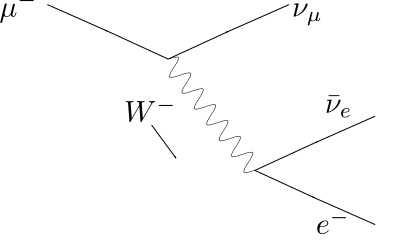
\includegraphics[scale=0.5]{muon_decay}
  \caption{diagrama de Feynman para el decaimiento $\mu^-\to \nu_\mu e^-\bar{\nu}_e$}
  \label{fig:muondecay}
\end{figure}
El propagador para el bos\'on $W$ de momentum $q$ resulta ser
\begin{align}
  \widetilde{D}_{\mu\nu}=\frac{1}{q^2-m_W^2}\left(g_{\mu\nu}-\frac{q_\mu q_\nu}{m_W^2}\right)\,.
\end{align}
Para los prop\'ositos actuales la obtenci\'on de este resultado no es necesaria, el punto importante es que cuando las masas de las part\'\i culas iniciales y finales son mucho m\'as peque\~nas que $m_W$, esto se reduce a
\begin{align}
  \widetilde{D}_{\mu\nu}=-\frac{g_{\mu\nu}}{m_W^2}\,.
\end{align}
Este resultado se entiende f\'acilmente cuando se compara con el propagador de una part\'\i culas escalar masiva $1/(q^2-M^2)\to-1/M^2$. Las componentes espaciales de $W_\mu$ con $\mu=1,2,3$, a bajas energ\'\i as tienen el mismo propagador que el de una part\'\i cula escalar, mientras $W_0$, tiene el signo opuesto.

El Lagrangiano efectivo para el decaimiento del mu\'on, $\mu^-\to \nu_\mu e^- \bar{\nu}_e$ es entonces
\begin{align}
  \mathcal{L}=&\frac{g^2}{8}\left[\bar{\nu}_\mu\gamma^\mu(1-\gamma_5)\mu\right]\frac{g_{\mu\nu}}{m_W^2}
  \left[\bar{e}\gamma^\nu(1-\gamma_5)\nu_e\right]\nonumber\\
=&\frac{g^2}{8m_W^2}\left[\bar{\nu}_\mu\gamma^\mu(1-\gamma_5)\mu\right]
  \left[\bar{e}\gamma^\nu(1-\gamma_5)\nu_e\right]\nonumber\\
  =&\frac{G_F}{\sqrt{2}}\left[\bar{\nu}_\mu\gamma^\mu(1-\gamma_5)\mu\right]\left[\bar{e}\gamma_\mu(1-\gamma_5)\nu_e\right]\,,
\end{align}
donde
\begin{align}
  \frac{G_F}{\sqrt{2}}=&\frac{g^2}{8m_W^2}\nonumber\\
  =&\frac{g^24}{8g^2v^2}\nonumber\\
  =&\frac{1}{2v^2}\,,
\end{align}
y
\begin{align}
  v=\left(\sqrt{2}G_F\right)^{-1/2}\,.
\end{align}


De otro lado, para el  decaimiento $\beta$, $n\to p e^- \bar{\nu}_e$, de acuerdo a la figura~\ref{fig:neutrondecay}, tenemos

\begin{align}
    \mathcal{L}=\frac{G_\beta}{\sqrt{2}}\left[\bar{p}\gamma^\mu(1-1.26\gamma_5)n\right]\left[\bar{e}\gamma_\mu(1-\gamma_5)\nu_e\right]\,.
\end{align}
\begin{figure}
  \centering
  \includegraphics[scale=0.5]{neutrondecay}
  \caption{Decaimiento del neutr\'on.}
  \label{fig:neutrondecay}
\end{figure}
con $G_F$ dado en la ec.~\eqref{eq:233} y $G_\beta=1.10\times10^{-5}\,\text{GeV}^2$. La corriente hadr\'onica tiene la forma V--1.26A. El factor 1.26  puede entenderse como debido a las correcciones a nivel hadr\'onico de una corriente que es de la forma V--A a nivel del quarks, como en la ec.~\eqref{eq:234}. A nivel de quarks el decaimiento del neutr\'on ($udd$) al prot\'on ($uud$) corresponde al decaimiento de uno de los quarks down del neutr\'on $d\to u e^- \bar{\nu}_e$
\begin{align}
    \mathcal{L}=\frac{G_F}{\sqrt{2}}V_{11}\left[\bar{u}\gamma^\mu(1-\gamma_5)d\right]\left[\bar{e}\gamma_\mu(1-\gamma_5)\nu_e\right]\,.
\end{align}
De modo que $G_\beta=G_F V_{11}=G_F\cos\theta_C$, donde $\theta_C$ es el \'angulo de Cabbibo. Una vez se tienen en cuenta correcciones electrod\'ebiles se obtiene el valor $|V_{11}|=0.97418(27)$\cite{PDG}. Las magnitudes de los elementos de la matriz CKM son\cite{PDG}
\begin{align}
  V\approx\begin{pmatrix}
    0.97419&0.2257&0.0359\\
    0.2256&0.97334&0.0415\\
    0.00874&0.0407&0.999133
  \end{pmatrix}\sim \mathbf{1}
\end{align}

\section{C\'alculo de procesos}
\label{sec:calculo-de-procesos}
Se remite al lector al lector a la siguiente parte del curso ``Standard Model and beyond'', de la p\'agina web 

\url{http://gfif.udea.edu.co:2500}

En particular a las secciones iniciales de los Cap\'\i tulos 1 y 2 donde se analizan el decaimiento $W^-\to e^-\bar{\nu}_e$ y el decaimiento del muon. 


\section{Problemas}
\label{sec:problemas-1}
\begin{enumerate}
\item Demuestre expl\'\i citamente la ec.~(\ref{eq:228})
\label{item:chap6.1}
\end{enumerate}


% \left(\right)
%
%%% Local Variables: 
%%% mode: latex
%%% TeX-master: "fullnotes"
%%% End: 
